% Options for packages loaded elsewhere
\PassOptionsToPackage{unicode}{hyperref}
\PassOptionsToPackage{hyphens}{url}
\PassOptionsToPackage{dvipsnames,svgnames*,x11names*}{xcolor}
%
\documentclass[
  a4paper, 11pt]{article}
\usepackage{lmodern}
\usepackage{amssymb,amsmath}
\usepackage{ifxetex,ifluatex}
\ifnum 0\ifxetex 1\fi\ifluatex 1\fi=0 % if pdftex
  \usepackage[T1]{fontenc}
  \usepackage[utf8]{inputenc}
  \usepackage{textcomp} % provide euro and other symbols
\else % if luatex or xetex
  \usepackage{unicode-math}
  \defaultfontfeatures{Scale=MatchLowercase}
  \defaultfontfeatures[\rmfamily]{Ligatures=TeX,Scale=1}
\fi
% Use upquote if available, for straight quotes in verbatim environments
\IfFileExists{upquote.sty}{\usepackage{upquote}}{}
\IfFileExists{microtype.sty}{% use microtype if available
  \usepackage[]{microtype}
  \UseMicrotypeSet[protrusion]{basicmath} % disable protrusion for tt fonts
}{}
\makeatletter
\@ifundefined{KOMAClassName}{% if non-KOMA class
  \IfFileExists{parskip.sty}{%
    \usepackage{parskip}
  }{% else
    \setlength{\parindent}{0pt}
    \setlength{\parskip}{6pt plus 2pt minus 1pt}}
}{% if KOMA class
  \KOMAoptions{parskip=half}}
\makeatother
\usepackage{xcolor}
\IfFileExists{xurl.sty}{\usepackage{xurl}}{} % add URL line breaks if available
\IfFileExists{bookmark.sty}{\usepackage{bookmark}}{\usepackage{hyperref}}
\hypersetup{
  pdftitle={Crítica ao uso do Campo de Arbítrio do Avaliador},
  pdfauthor={Luiz F. P. Droubi; Carlos Augusto Zilli; Willian Zonato; Norberto Hochheim},
  colorlinks=true,
  linkcolor=red,
  filecolor=Maroon,
  citecolor=green,
  urlcolor=magenta,
  pdfcreator={LaTeX via pandoc}}
\urlstyle{same} % disable monospaced font for URLs
\usepackage[left=2.5cm,right=2.5cm,top=3cm,bottom=2.5cm]{geometry}
\usepackage{longtable,booktabs}
% Correct order of tables after \paragraph or \subparagraph
\usepackage{etoolbox}
\makeatletter
\patchcmd\longtable{\par}{\if@noskipsec\mbox{}\fi\par}{}{}
\makeatother
% Allow footnotes in longtable head/foot
\IfFileExists{footnotehyper.sty}{\usepackage{footnotehyper}}{\usepackage{footnote}}
\makesavenoteenv{longtable}
\usepackage{graphicx,grffile}
\makeatletter
\def\maxwidth{\ifdim\Gin@nat@width>\linewidth\linewidth\else\Gin@nat@width\fi}
\def\maxheight{\ifdim\Gin@nat@height>\textheight\textheight\else\Gin@nat@height\fi}
\makeatother
% Scale images if necessary, so that they will not overflow the page
% margins by default, and it is still possible to overwrite the defaults
% using explicit options in \includegraphics[width, height, ...]{}
\setkeys{Gin}{width=\maxwidth,height=\maxheight,keepaspectratio}
% Set default figure placement to htbp
\makeatletter
\def\fps@figure{htbp}
\makeatother
\setlength{\emergencystretch}{3em} % prevent overfull lines
\providecommand{\tightlist}{%
  \setlength{\itemsep}{0pt}\setlength{\parskip}{0pt}}
\setcounter{secnumdepth}{5}
\usepackage[brazil]{babel}
%\usepackage{titling}
\usepackage{amsmath}
\usepackage{graphicx}
\usepackage{float}
\usepackage{subfig}
\usepackage{caption}
\usepackage{lastpage}
\usepackage{rotating}
\usepackage{mathrsfs}
\usepackage{bm}
\usepackage{dcolumn}
\setlength{\parindent}{1.25cm} % Default is 15pt.
\usepackage{indentfirst}
% \usepackage{helvet}
% \renewcommand{\familydefault}{\sfdefault}
% \usepackage{newtxtext,newtxmath} % mais nova para Times.
%\usepackage{mathptmx} % para Times New Roman (preferível newtxtext)
% \usepackage{Times} % para Times New Roman (obsoleto)
\usepackage{fontspec} % para Arial e/ou Times (xelatex ou luatex)
\setmainfont{Arial}
\newcommand{\pkg}[1]{{\normalfont\fontseries{b}\selectfont #1}}
\let\proglang=\textsf
\let\code=\texttt
\usepackage{fancyhdr}
% Turn on the style
\pagestyle{fancy}
\fancyhf{}
% Clear the header and footer
\fancyhead{}
\fancyfoot{}
% Set the right side of the footer to be the page number
\fancyhead[CO, CE]{
  \textbf{IX SIMPÓSIO DA SOCIEDADE BRASILEIRA DE ENGENHARIA DE AVALIAÇÕES}
}
\fancyfoot[CO, CE]{\textbf{Crítica ao uso do Campo de Arbítrio do Avaliador}}
\fancyfoot[R]{\thepage~/~\pageref{LastPage}}
\usepackage{booktabs}
\usepackage{longtable}
\usepackage{array}
\usepackage{multirow}
\usepackage{wrapfig}
\usepackage{float}
\usepackage{colortbl}
\usepackage{pdflscape}
\usepackage{tabu}
\usepackage{threeparttable}
\usepackage{threeparttablex}
\usepackage[normalem]{ulem}
\usepackage{makecell}

\title{Crítica ao uso do Campo de Arbítrio do Avaliador}
\usepackage{etoolbox}
\makeatletter
\providecommand{\subtitle}[1]{% add subtitle to \maketitle
  \apptocmd{\@title}{\par {\large #1 \par}}{}{}
}
\makeatother
\subtitle{Devido à escassez de dados de mercado}
\author{Luiz F. P. Droubi\footnote{SPU/SC,
  \href{mailto:lfpdroubi@gmail.com}{\nolinkurl{lfpdroubi@gmail.com}}} \and Carlos Augusto Zilli\footnote{IFSC,
  \href{mailto:carlos.zilli@ifsc.edu.br}{\nolinkurl{carlos.zilli@ifsc.edu.br}}} \and Willian Zonato\footnote{SPU/SC,
  \href{mailto:will.zonato@gmail.com}{\nolinkurl{will.zonato@gmail.com}}} \and Norberto Hochheim\footnote{UFSC,
  \href{mailto:hochheim@gmail.com}{\nolinkurl{hochheim@gmail.com}}}}
\date{15/10/2020}

\begin{document}
\maketitle

\hypertarget{resumo}{%
\section*{Resumo}\label{resumo}}
\addcontentsline{toc}{section}{Resumo}

Neste trabalho são apresentados aspectos teóricos e práticos
relacionados ao conceito de Campo de Arbítrio (CA) do Avaliador, dada a
importância deste conceito na Engenharia de Avaliações. Foram elencados
os critérios previstos na normativa que possibilitam ao avaliador fazer
uso do Campo de Arbítrio, detalhando cada um destes critérios levantados
e ponderando se a adoção do conceito de Campo de Arbítrio do avaliador é
uma condição suficiente e necessária para a solução dos problemas
práticos enfrentados pelo avaliador. Para melhor ilustrar, foram
elaborados estudos de diversos casos com a geração de dados randômicos
simulando o problema da micronumerosidade de dados de uma mesma
característica, comparando os resultados obtidos com a adoção de
diversas abordagens, fazendo uso tanto do Campo de Arbítrio do Avaliador
quando do intervalo de predição (IP) das previsões efetuadas com os
modelos obtidos em cada abordagem. Outro aspecto importante abordado
lateralmente neste trabalho é sobre a previsão de valores de venda a
partir de dados de oferta, haja vista que a falta de dados de transações
e, em consequência a falta de um fator oferta obtido cientificamamente,
é um dos grandes motivos que levam os avaliadores a fazerem uso do Campo
de Arbítrio. Ao final, a partir da pesquisa elaborada e dos resultados
obtidos são feitas recomendações visando uma melhoria na NBR 14.653 numa
eventual revisão desta.

\hypertarget{introduuxe7uxe3o}{%
\section{Introdução}\label{introduuxe7uxe3o}}

No \href{http://www.cobreap.com.br/2019/}{XX Cobreap}, foi apresentado o
artigo intitulado ``Crítica à Avaliação Intervalar na NBR14.653-02''
(DROUBI et al., \protect\hyperlink{ref-droubi2019}{2019}). Neste
trabalho recomendou-se que, eventualmente, em uma próxima revisão da
parte 2 da NBR 14.653-02 (\protect\hyperlink{ref-NBR1465302}{2011}), a
avaliação intervalar, tal como está normatizada no momento, não seja
mantida como se encontra. Com base nos resultados obtidos naquele
artigo, foram elaborados outros estudos, com ajustes diferentes, com o
intuito de verificar a pertinência das conclusões obtidas naquele
trabalho, assim como acrescentar alguns pontos no que tange ao Campo de
Arbítrio do avaliador, especialmente em relação à omissão de variável
relevante. Também foram feitas considerações a respeito do fator oferta.
Pretende-se com este trabalho deixar detalhes de uma proposta de como
poder-se-ia modificar o atual consenso da avaliação intervalar numa
futura revisão normativa.

\hypertarget{desenvolvimento-e-fundamentauxe7uxe3o}{%
\section{Desenvolvimento e
Fundamentação}\label{desenvolvimento-e-fundamentauxe7uxe3o}}

Nesta seção serão abordados o conceito básico de campo de arbítrio, como
definido pela ABNT (\protect\hyperlink{ref-NBR1465302}{2011}), o
conceito de viés devido à omissão de variável relevante, tal como prevê
o campo de arbítrio, além de questões correlatas, como a questão do
sobreajuste (\emph{overfitting}) em modelos estatísticos e o
\emph{tradeoff} entre viés e variância.

\hypertarget{campo-de-arbuxedtrio-do-avaliador}{%
\subsection{Campo de Arbítrio do
Avaliador}\label{campo-de-arbuxedtrio-do-avaliador}}

A NBR 14.653-02 (ABNT, \protect\hyperlink{ref-NBR1465302}{2011}) define
que:

\begin{quote}
``\emph{o Campo de Arbítrio pode ser utilizado quando \textbf{variáveis
relevantes} para a avaliação do imóvel \textbf{não tiverem sido
contempladas no modelo}, por escassez de dados de mercado, por
inexistência de fatores de homogeneização aplicáveis ou porque essas
variáveis não se apresentaram estatisticamente significantes em modelos
de regressão, \textbf{desde que a amplitude de até mais ou menos 15\%
seja suficiente para absorver as influências não consideradas e que os
ajustes sejam justificados}}''.
\end{quote}

Um ponto levantado por Droubi \emph{et al.}
(\protect\hyperlink{ref-droubi2019}{2019}) é que a comparação dos
valores arbitrados dentro do CA não deveriam ser comparados ao intervalo
de confiança da regressão linear, pois \emph{o intervalo de confiança é
para a média}, ou seja, o intervalo de confiança é apenas para aferir a
precisão do cálculo dos valores ajustados pela reta de regressão (média
+ variância explicada) e não serve para contemplar outros efeitos não
calculados pelo modelo para a avaliação do bem-avaliando. Para isto, a
comparação devida seria com o intervalo de predição, ou seja, o
intervalo onde se encontram os valores reais observados do mercado e não
apenas os valores médios (a soma da média e da variância explicada e
não-explicada).

Este primeiro aspecto refere-se mais à questão da avaliação intervalar
do que ao campo de arbítrio em si, e poderia ser contornado simplesmente
com a mudança dos critérios da avaliação intervalar, adotando-se
critérios mais adequados para a elaboração de intervalos.

Um outro ponto igualmente importante levanto por Droubi \emph{et al.}
(\protect\hyperlink{ref-droubi2019}{2019}), porém, diz respeito apenas
ao CA: o intervalo fixo, de \(\pm\) 15\%, pode até ser razoável em
algumas situações, mas pode levar a valores de baixíssima probabilidade
de ocorrência prática em mercados de baixa variabilidade, ou ainda, pelo
contrário, num mercado de grande variância, levar a valores que sequer
chegam próximos dos valores extremos observados no mercado.

Porém, entende-se que Droubi \emph{et al.}
(\protect\hyperlink{ref-droubi2019}{2019}) não esclareceram
completamente os motivos pelos quais um modelo pode vir a apresentar um
intervalo de predição tão grande, enquanto noutros o intervalo de
predição pode ser mais estreito.

Como será visto a seguir, isto pode ser uma questão relacionada apenas
ao próprio mercado, como defenderam Droubi \emph{et al.}
(\protect\hyperlink{ref-droubi2019}{2019}), mas também pode estar
relacionado às variáveis importantes não contempladas no modelo. Na
próxima subseção será analisado um dos fatores que podem levar à omissão
de variáveis importantes num modelo de avaliação de imóveis.

\hypertarget{escassez-de-dados-de-mercado---micronumerosidade}{%
\subsection{Escassez de dados de mercado -
Micronumerosidade}\label{escassez-de-dados-de-mercado---micronumerosidade}}

Um dos fatores que levam à omissão de variáveis relevantes do modelo, o
que embasa a utilização do CA do avaliador, é o critério da
micronumerosidade.

De acordo com o Anexo A da referida norma, quando da utilização de
variáveis dicotômicas ou qualitativas, um número mínimo de dados de cada
característica, variando de 3 a 10, a depender do tamanho da amostra,
devem ser efetivamente utilizados. Em geral, o número de dados de cada
característica (\(n_i\)) deve ser igual a 10\% do número total de dados
(\(n_i \geq 10\% \ n\)) da amostra, limitado a um mínimo de 3 dados caso
a amostra possua um número total de dados menor do que 30 (\(n<30\)) e
um limitante superior de 10 dados \(n_i \geq 10\) caso a amostra possua
um número de dados maior do que 100 (\(n > 100\)).

A NBR 14.653-02 não é clara, no entanto, sobre como proceder no caso de
o avaliador encontrar em sua amostra um número de dados de uma
característica menor do que o mínimo estabelecido. Existem diversas
possibilidades, como:

\begin{enumerate}
\def\labelenumi{\alph{enumi}.}
\tightlist
\item
  a remoção da variável que apresenta a micronumerosidade;
\item
  a recodificação da variável (quando possível);
\item
  a remoção dos dados que apresentam aquela característica em número
  insuficiente.
\end{enumerate}

A depender do procedimento adotado, o avaliador obterá um modelo
diferente e a implicância da adoção de cada procedimento será mostrada
nos estudos de casos apresentados. Presume-se, no entanto, a partir de
uma leitura global da norma, que a mesma sugere que a variável
\textbf{e} os dados sejam removidos do modelo, pois com a remoção apenas
da variável e a inclusão dos dados com características diferentes no
modelo, a hipótese da homoscedasticidade dos resíduos, normalmente, não
se verifica, como será mostrado, e a norma também veda a utilização de
modelos em que as hipóteses da inferência clássica não se cumpram, de
acordo com o \emph{caput} do item A.2.

\hypertarget{inexistuxeancia-de-fatores-de-homogeneizauxe7uxe3o}{%
\subsection{Inexistência de fatores de
homogeneização}\label{inexistuxeancia-de-fatores-de-homogeneizauxe7uxe3o}}

Ficou claro durante o \href{http://www.cobreap.com.br/2019/}{XX Cobreap}
que grande parte dos avaliadores se utiliza do CA para resolver um dos
maiores problemas da prática atual da Engenharia de Avaliações, que é a
falta de dados de transações, o que implica na impossibilidade do
cálculo de um fator oferta. A imensa maioria dos Avaliadores se valem de
uma pesquisa de dados ofertados, chegando assim a um modelo para os
preços de oferta, que infelizmente não corresponde a um modelo de preços
de venda dos imóveis.

A atual normativa não permite a aplicação de um fator oferta aos dados
pesquisados, a menos que este fator seja deduzido com a utilização de
metodologia científica.

No entanto, um modelo econométrico proposto por Horowitz
(\protect\hyperlink{ref-horowitz}{1992}) permite a previsão de preços de
venda a partir de preços de oferta mais precisamente do que os que
seriam obtidos com um modelo hedônico elaborado à partir dos próprios
dados de venda.

Num estudo de caso Horowitz (\protect\hyperlink{ref-horowitz}{1992}, pp.
124--125), encontrou um modelo econométrico que previu os preços de
vendas a partir dos preços de oferta com um erro médio quadrático de
apenas \$2.960, enquanto que com um modelo hedônico elaborado a partir
dos próprios dados de venda foi obtido um erro de \$10.361, ou seja, um
erro médio muito maior do que o erro médio obtido com o modelo
econométrico proposto.

Está fora do escopo deste trabalho detalhar a abordagem de Horowitz
(\protect\hyperlink{ref-horowitz}{1992}). Contudo, a existência de um
método capaz de prever preços de venda de imóveis a partir apenas de
dados de oferta, e com melhor precisão do que um modelo hedônico
elaborado com os próprios dados de venda é um fator a menos em favor da
utilização do CA do avaliador com esta finalidade. Estudos devem ser
levados a cabo e possivelmente o modelo tenha que ser adaptado para se
ajustar à realidade da prática da Engenharia de Avaliações no Brasil,
porém a existência de tal abordagem não pode permanecer completamente
ignorada como é hoje na Engenharia de Avaliações.

\hypertarget{falta-de-significuxe2ncia-dos-regressores}{%
\subsection{Falta de significância dos
regressores}\label{falta-de-significuxe2ncia-dos-regressores}}

Um dos pontos polêmicos da NBR 14.653-02 consiste na adoção de graus de
fundamentação de modelos de regressão linear. Entre os critérios
utilizados para o enquadramento dos modelos nos diversos graus de
fundamentação está o nível de significância máxima para a rejeição da
hipótese nula de cada regressor. Está além do escopo deste artigo uma
crítica pormenorizada a este critério, porém deve-se salientar que este
tipo de análise de importância de regressores à partir dos p-valores dos
testes de hipótese tem sido muito contestada entre os estatísticos (ver
MATLOFF, \protect\hyperlink{ref-matloff2017}{2017}, p. 349; WASSERSTEIN;
LAZAR, \protect\hyperlink{ref-ASA}{2016}).

\hypertarget{viuxe9s-devido-uxe0-omissuxe3o-de-variuxe1vel}{%
\subsection{Viés devido à omissão de
variável}\label{viuxe9s-devido-uxe0-omissuxe3o-de-variuxe1vel}}

Nesta subseção serão apresentados aspectos teóricos a respeito da
omissão de variáveis relevantes de um modelo de regressão,
independentemente dos motivos que levem a esta omissão, seja por
escassez de dados de mercado, seja por falta de significância do
regressor.

Segundo Matloff (\protect\hyperlink{ref-matloff2017}{2017}, p. 24),
adicionando mais variáveis independentes a um modelo se está a reduzir o
viés do modelo.

Em tese, qualquer coisa que influencie o valor da variável dependente e
não esteja presente no modelo é absorvido pelo termo de erro (variação
não-explicada pelo modelo), que se assume estar não-correlacionado com
os regressores (\(\mathbb{E}[\varepsilon|X] = 0\)). No entanto, se
houver algum grau de correlação entre a variável omitida e as variáveis
presentes, como os efeitos da variável omitida são absorvidas pelo termo
de erro, a hipótese de independência dos resíduos não será mantida.
Segundo Matloff (\protect\hyperlink{ref-matloff2017}{2017}, p. 25), um
modelo assim é chamado pelos economistas de modelo mal-especificado
(\emph{misspecified}), enquanto os estatísticos tratam este de tipo viés
como viés de modelagem (\emph{model bias}).

De acordo com Matloff (\protect\hyperlink{ref-matloff2017}{2017}, p.
25), no entanto, isto não quer dizer que se trata de um viés que tenha
sido adicionado deliberadamente ao modelo, apenas quer dizer que existe
no modelo um viés sistêmico, que é permanente e não desaparece, por mais
que aumente-se o tamanho da amostra.

\hypertarget{sobreajuste}{%
\subsection{Sobreajuste}\label{sobreajuste}}

O sobreajuste ou \emph{overfitting} em estatística é uma prática que
consiste em elaborar um modelo qualquer de maneira tão complexa que, ao
invés de captar o sinal, capta o ruído (MATLOFF,
\protect\hyperlink{ref-matloff2017}{2017}, p. 24).

A prática, então, de se adicionar variáveis ao modelo para reduzir o
viés da estimação, como visto na subseção anterior, tem um limite: a
introdução de uma variável, ao diminuir o viés, também aumenta a
variância das estimativas dos coeficientes do modelo. Em um determinado
ponto, o benefício da adição de variáveis ao modelo será menor do que a
maior variabilidade que ocorrerá na estimação, o que é chamado de
\emph{overfitting} (MATLOFF, \protect\hyperlink{ref-matloff2017}{2017},
p. 24).

Segundo Matloff (\protect\hyperlink{ref-matloff2017}{2017}, p. 24), para
qualquer estimador estatístico \(\hat \theta\) com variância finita,
pode ser mostrado que:

\begin{equation} \label{eq:tradeoff}
MSE(\hat \theta) = Var(\hat \theta) + B^2(\hat \theta)
\end{equation}

Onde \(MSE(\hat\theta)\) é o erro médio quadrático associado ao
estimador, \(Var(\hat\theta)\) é a variância do estimador e
\(B^2(\hat\theta)\) é o quadrado do viés do estimador.

Segundo Matloff (\protect\hyperlink{ref-matloff2017}{2017}, p. 25), a
equação \ref{eq:tradeoff} mostra que, adicionando variáveis ao estimador
de regressão linear, reduz-se o termo \(B^2(\hat \theta)\), porém ao
custo do aumento da variância (\(Var(\hat\theta)\)) e vice-versa, ao se
remover variáveis do modelo, se está aumentando o viés do modelo,
reduzindo, porém sua variância. De acordo com Matloff pode ser até
benéfico remover variáveis de um modelo com o intuito de reduzir a
variância do estimador, ao custo de aceitar um pouco de viés (MATLOFF,
\protect\hyperlink{ref-matloff2017}{2017}, p. 25).

Um bom exemplo para o entendimento do problema pode ser encontrado em
MATLOFF (\protect\hyperlink{ref-matloff2017}{2017}, pp. 342--343),
reproduzido abaixo:

Supondo uma amostra com alturas de meninos e meninas, estimar as alturas
médias de ambas as populações, com variância conhecida igual a
\(\sigma^2\). De acordo com Matloff, os estimadores naturais seriam:

\begin{equation} \label{eq:boysandgirls}
\hat\mu_1 = \frac{1}{n}\sum_{i=1}^{n}X_i \qquad e \qquad \hat\mu_2 = \frac{1}{n}\sum_{i=1}^{n}Y_i
\end{equation}

Porém, se o número de dados da amostra é pequeno, pode ser melhor
simplificar o modelo e utilizar um único estimador para ambos os grupos:

\begin{equation} \label{eq:all}
\check \mu_i = \frac{1}{2}(\bar X + \bar Y), \ i = 1,2
\end{equation}

O critério para a escolha do melhor estimador é o erro médio quadrático
(MSE).

Ocorre que o erro médio quadrático para os estimadores das equações
\ref{eq:boysandgirls} é igual à variância dos estimadores, dado que
ambos são estimadores não-viesados
(\(B(\hat \mu_1) = B(\hat \mu_2) = 0\)):

\begin{equation} \label{eq:mse1}
MSE(\hat\mu_1) + MSE(\hat\mu_2) = 2 Var(\hat \mu_i) = 2 \frac{\sigma^2}{n}
\end{equation}

Já para os estimadores \(\check \mu_i\) a soma dos seus erros médios
quadráticos pode ser vista na equação \ref{eq:mse2}\footnote{Obtido
  através da soma das variâncias e viés quadrados dos estimadores, como
  pode ser visto em MATLOFF (\protect\hyperlink{ref-matloff2017}{2017},
  pp. 386--387).}

\begin{equation} \label{eq:mse2}
MSE(\check\mu_1) + MSE(\check\mu_2) = \frac{\sigma^2}{n} + \frac{1}{2}(\mu_1 - \mu_2)^2
\end{equation}

Desta maneira, para saber qual o melhor estimador, deve-se comparar os
valores dos erros médios quadráticos obtidos nas equações \ref{eq:mse1}
e \ref{eq:mse2}.

Caso \(2\frac{\sigma^2}{n} < (\mu_1-\mu_2)^2\), adotam-se os estimadores
naturais. Caso contrário, mais vale a pena adotar o estimador único para
ambos os grupos.

Deve-se ter em conta que:

\begin{enumerate}
\def\labelenumi{\arabic{enumi}.}
\tightlist
\item
  se a diferença entre as médias \(\mu_1\) e \(\mu_2\) é pequena, o
  estimador único é bem próximo da realidade;
\item
  se o número de dados \(n\) é pequeno, não há dados suficientes para se
  estimar com precisão os dois estimadores em separado;
\item
  se a variância da população é alta, também será preciso mais dados
  para a estimação em separado das duas médias.
\end{enumerate}

Segundo Matloff (\protect\hyperlink{ref-matloff2017}{2017}, p. 344),
este exemplo é um problema trivial de regressão, onde deve-se escolher
entre um modelo nulo (\(p = 0\)), e um modelo mais elaborado, com um
regressor (\(p = 1\)), a saber, a variável dicotômica que indica se
tratar de um dado de altura de menino ou menina.

Ainda de acordo com Matloff (\protect\hyperlink{ref-matloff2017}{2017},
p. 344), isto pode ser estendido ao contexto genérico de modelos de
regressão e classificação, com \(p\) regressores e \(n\) observações: se
\(p\) é grande e/ou \(n\) é pequeno, pode ser desejável utilizar um
modelo mais simples, omitindo alguns regressores em que o valor de
\(\beta\) seja negligenciável.

De acordo com Tukey e outro trabalho mais recente de Portnoy
(\emph{apud} MATLOFF, \protect\hyperlink{ref-matloff2017}{2017}, p.
344), via de regra, devem existir no máximo \(\sqrt{n}\) regressores em
um modelo de regressão para se evitar o sobreajuste do modelo.

\hypertarget{estudos-de-casos}{%
\section{Estudos de Casos}\label{estudos-de-casos}}

Neste trabalho foram elaborados dois estudos de casos.

No primeiro estudo de caso, que visa explorar os efeitos da omissão de
variáveis relevantes nos modelos de regressão linear, foram feitas
quatro simulações, variando o efeito da majoração dos valores de lotes
em situação de esquina, em relação aos lotes em situação de meio de
quadra.

Foi elaborado ainda um segundo estudo de caso visando obter reflexões
acerca da utilização do CA quando, pelo contrário, não existem variáveis
\textbf{relevantes} omitidas, ainda que haja variabilidade na amostra, o
que também é normal que aconteça.

\hypertarget{estudo-de-caso-1-viuxe9s-devido-uxe0-omissuxe3o-de-variuxe1vel-relevante}{%
\subsection{Estudo de Caso 1 -- Viés devido à omissão de variável
relevante}\label{estudo-de-caso-1-viuxe9s-devido-uxe0-omissuxe3o-de-variuxe1vel-relevante}}

Neste Estudo de Caso foram elaborados quatro simulações de dados
aleatórios para discussão de alguns fatos que são ilustrados com a
aplicação de diferentes abordagens para o tratamento dos dados.

Para os quatro casos, os dados do Valor Unitário de cada lote (VU) foram
criados através da seguinte equação de regressão (da população),
conforme equação \ref{eq:generic}:

\begin{equation} \label{eq:generic}
VU = \beta_0 + \beta_1 \cdot Area + \beta_2 \cdot Situacao + \varepsilon
\end{equation}

Onde \(\varepsilon \sim \mathcal{N}(0, \sigma^2)\). Para os diversos
casos foram variados os valores dos coeficientes da população
\(\beta_i\) utilizados para a geração de dados, de maneira a salientar o
comportamento dos diversos modelos ajustados tanto na estimação dos
coeficientes (\(\hat\beta_i\)), quando na elaboração de previsões sobre
um lote de referência.

A vantagem de se trabalhar com dados gerados é que se conhece \emph{a
priori} o valor dos coeficientes (\(\beta_i\)) da população, já que
estes estão pré-definidos. Obviamente que, com a inclusão de um ruído
(\(\varepsilon\)), no ajuste dos modelos de regressão aos dados gerados,
não são obtidos para os coeficientes ajustados (\(\hat \beta_i\))
exatamente os mesmos valores dos coeficientes populacionais
(\(\beta_i\)) utilizados para a geração dos dados. Mas se o modelo
estiver bem especificado, os valores estimados para os coeficientes
devem ser próximos dos coeficientes utilizados para a geração dos dados,
ou seja, \(\hat \beta_i \approx \beta_i\).

Em todos os casos foram gerados dados (propositalmente) em número
insuficiente (\(<3\)) para o caso dos lotes em situação de esquina.

Foram estudadas, então, as consequências da utilização de três
diferentes tipos de abordagens:

\begin{itemize}
\item
  O ajuste de um modelo de regressão com a inclusão de todos os dados,
  porém com a omissão da variável \texttt{situacao}, visando emular o
  caso previsto na definição de CA, de omissão de variável relevante do
  modelo devido à escassez de dados de mercado;
\item
  O ajuste de um modelo de regressão com a exclusão dos dados de
  esquina, de maneira a se obter um modelo ajustado em cima de uma
  amostra homogênea, isto é, um amostra onde todos os dados possuem as
  mesmas características em relação à variável \texttt{situacao}.
\item
  O ajuste de um modelo de regressão com a inclusão de todos os dados e
  todas as variáveis, apesar da recomendação em contrário da NBR
  14.653-02.
\end{itemize}

\hypertarget{mercado-1}{%
\subsubsection{Mercado 1}\label{mercado-1}}

\begin{wraptable}{r}{0pt}[ht]
\centering
\begin{tabular}{ccc}
  \hline
VU & Area & Situacao \\ 
  \hline
\cellcolor{gray!6}{3137} & \cellcolor{gray!6}{360} & \cellcolor{gray!6}{Meio de Quadra }\\ 
  3218 & 360 & Meio de Quadra \\ 
\cellcolor{gray!6}{  3116} & \cellcolor{gray!6}{360} & \cellcolor{gray!6}{Meio de Quadra }\\ 
  3360 & 360 & Meio de Quadra \\ 
\cellcolor{gray!6}{  2883} & \cellcolor{gray!6}{480} & \cellcolor{gray!6}{Esquina }\\ 
  2768 & 480 & Esquina \\ 
\cellcolor{gray!6}{  3249} & \cellcolor{gray!6}{360} & \cellcolor{gray!6}{Meio de Quadra }\\ 
  3274 & 360 & Meio de Quadra \\ 
\cellcolor{gray!6}{  2658} & \cellcolor{gray!6}{480} & \cellcolor{gray!6}{Meio de Quadra }\\ 
  2569 & 480 & Meio de Quadra \\ 
   \hline
\end{tabular}
\caption{Dados para o M. 1.} 
\label{tab:ex1}
\end{wraptable}

Para este exemplo os dados foram gerados através da equação
\ref{eq:ex1}, onde \(\varepsilon \sim \mathcal{N}(0, \,100^2)\):

\begin{equation} \label{eq:ex1}
VU = 5000 - 5 \cdot Area + 250 \cdot Situacao + \varepsilon
\end{equation}

Seja o caso de se avaliar um lote urbano de esquina com 480\(m^2\),
baseado na amostra exibida na tabela \ref{tab:ex1}, obtida com as
simulações, onde \texttt{Situacao} é uma variável dicotômica que
diferencia os imóveis em situação de meio de quadra (0) dos imóveis de
esquina (1).

De acordo com a NBR 14.653-02, como estão disponíveis apenas 2 dados de
mercado em situação de esquina, não seria possível a utilização da
variável \texttt{Situacao}, devido à micronumerosidade. Neste tipo de
situação (escassez de dados de mercado), a norma permite a utilização do
CA.

Ou seja, segundo a NBR 14.653-02 leva a crer, poderia ser elaborado um
modelo com todos os dados amostrais, com a inclusão apenas da variável
\texttt{Area}, omitindo-se a variável \texttt{Situacao} e utilizar o CA
para majorar o valor estimado do lote pelo modelo, por este estar em
situação de esquina, \emph{desde que a amplitude de até mais ou menos
15\% seja suficiente para absorver as influências não consideradas e que
os ajustes sejam justificados}.

\begin{table}[H] \centering 
  \caption{Comparação de modelos para o Ex. 1.} 
  \label{tab:tab1} 
\footnotesize 
\begin{tabular}{@{\extracolsep{5pt}}lccc} 
\\[-1.8ex]\hline 
\hline \\[-1.8ex] 
 & \multicolumn{3}{c}{\textit{Dependent variable:}} \\ 
\cline{2-4} 
\\[-1.8ex] & \multicolumn{3}{c}{VU} \\ 
\\[-1.8ex] & (1) & (2) & (3)\\ 
\hline \\[-1.8ex] 
 Constant & 4.744,4 (4.433,2, 5.055,6) & 5.062,3 (4.767,0, 5.357,5) & 5.062,3 (4.769,3, 5.355,3) \\ 
  & t = 19,5$^{***}$ & t = 22,0$^{***}$ & t = 22,1$^{***}$ \\ 
  Area & $-$4,2 ($-$5,0, $-$3,5) & $-$5,1 ($-$5,9, $-$4,4) & $-$5,1 ($-$5,8, $-$4,4) \\ 
  & t = $-$7,2$^{***}$ & t = $-$8,7$^{***}$ & t = $-$8,8$^{***}$ \\ 
  SituacaoEsquina &  &  & 211,9 (102,5, 321,4) \\ 
  &  &  & t = 2,5$^{***}$ \\ 
 \hline \\[-1.8ex] 
Observations & 10 & 8 & 10 \\ 
R$^{2}$ & 0,9 & 0,9 & 0,9 \\ 
Adjusted R$^{2}$ & 0,8 & 0,9 & 0,9 \\ 
Residual Std. Error & 109,5 (df = 8) & 86,1 (df = 6) & 85,4 (df = 7) \\ 
F Statistic & 51,3$^{***}$ (df = 1; 8) & 75,9$^{***}$ (df = 1; 6) & 45,2$^{***}$ (df = 2; 7) \\ 
\hline 
\hline \\[-1.8ex] 
Notas: & \multicolumn{3}{r}{$^{*}$p$<$0,3; $^{**}$p$<$0,2; $^{***}$p$<$0,1} \\ 
\end{tabular} 
\end{table}

Na tabela \ref{tab:tab1} são mostrados os coeficientes dos três modelos
ajustados, isso fica claro: no primeiro modelo (coluna 1), foram
utilizados todos os dados e apenas a variável \texttt{Area}; no segundo
modelo (coluna 2), foram utilizados apenas os dados em situação de
meio-de-quadra; e no terceiro modelo (coluna 3) foram utilizados todos
os dados e foi incluída a variável \texttt{Situacao}, apesar da
micronumerosidade.

O que se percebe é que o primeiro modelo viesou para cima o coeficiente
da variável \texttt{Area}. Ou seja, o efeito da \texttt{Situacao} do
lote, que não foi incluso no modelo, foi ``absorvido'' pela outra
variável restante, ou seja, a variável \texttt{Area}. Isto ocorre porque
a modelagem não respeitou um dos princípios da inferência clássica, que
é a homogeneidade da amostra, haja vista que a amostra utilizada mistura
imóveis em situação de meio de quadra e imóveis em situação de esquina,
sem uma variável que modele esta diferença entre os dados amostrais.

Os outros dois modelos se aproximaram melhor dos coeficientes ``reais''
de regressão, ou seja, o valor dos coeficientes para a população ( 5000,
-5,0 e 250). Isto se deve à homogeneidade da amostra, obtida ou através
da exclusão dos dados não-homogêneos, ou com a inclusão de todos os
dados e variáveis relevantes, em que pese estar em desacordo com o
estabelecido pela NBR 14653-02. Deve-se notar, contudo, que a estimação
foi melhor para os coeficientes obtidos com o terceiro modelo, haja
vista o maior número de dados.

Pelo lado da estimação dos coeficientes, portanto, não se recomenda a
utilização da primeira abordagem. A segunda abordagem é preferível à
primeira, porém a terceira abordagem é ainda mais precisa que a segunda.

Com a primeira abordagem (o modelo da coluna 1), onde foram misturados
dados de esquina e de meio de quadra, esperava-se desvios em relação à
homoscedasticidade dos resíduos. No entanto, provavelmente devido à
pequena diferença entre os valores dos lotes em situação de esquina e
dos lotes em situação de meio de quadra, a hipótese da
homoscedasticidade não pôde ser rejeitada via teste de Breusch-Pagan:

\begin{verbatim}
## 
##  studentized Breusch-Pagan test
## 
## data:  fit_a
## BP = 1.4212, df = 1, p-value = 0.2332
\end{verbatim}

A tabela 3 apresenta o comportamento das diversas abordagens para a
previsão de novos valores com a utilização dos modelos ajustados. Nesta
tabela podem ser vistos os valores para a estimativa central e para os
limites inferiores e superiores do IP (@80\%) e do CA, assim como os
limites do CA. O valor teórico, obtido utilizando-se os coeficientes de
regressão para a população (\(\beta_i\)) seria de R\$2.850,00.

Percebe-se desta maneira que para o \textbf{primeiro modelo}, o valor
adicional do lote em esquina já foi absorvido e já se encontra, em
grande parte, na estimativa central efetuada com o mesmo. No
\textbf{segundo modelo}, que é um modelo feito apenas para os dados de
lotes em situação de meio de quadra, não há qualquer influência de lotes
em situação de esquina, ficando a previsão de valores para lotes de
esquina comprometida. E o \textbf{terceiro modelo}, apesar da
micronumerosidade, foi o que melhor estimou o lote em situação de
esquina.

\begin{longtable}[]{@{}lrrrrrr@{}}
\caption{Comparação dos limites do IP e CA para os modelos do Ex.
1.}\tabularnewline
\toprule
\begin{minipage}[b]{0.06\columnwidth}\raggedright
Abordagem\strut
\end{minipage} & \begin{minipage}[b]{0.14\columnwidth}\raggedleft
Estimativa central\strut
\end{minipage} & \begin{minipage}[b]{0.14\columnwidth}\raggedleft
\(IP_{inf}\)\strut
\end{minipage} & \begin{minipage}[b]{0.15\columnwidth}\raggedleft
\(IP_{sup}\)\strut
\end{minipage} & \begin{minipage}[b]{0.10\columnwidth}\raggedleft
Amplitude IP (\%)\strut
\end{minipage} & \begin{minipage}[b]{0.11\columnwidth}\raggedleft
\(CA_{inf}\)\strut
\end{minipage} & \begin{minipage}[b]{0.11\columnwidth}\raggedleft
\(CA_{sup}\)\strut
\end{minipage}\tabularnewline
\midrule
\endfirsthead
\toprule
\begin{minipage}[b]{0.06\columnwidth}\raggedright
Abordagem\strut
\end{minipage} & \begin{minipage}[b]{0.14\columnwidth}\raggedleft
Estimativa central\strut
\end{minipage} & \begin{minipage}[b]{0.14\columnwidth}\raggedleft
\(IP_{inf}\)\strut
\end{minipage} & \begin{minipage}[b]{0.15\columnwidth}\raggedleft
\(IP_{sup}\)\strut
\end{minipage} & \begin{minipage}[b]{0.10\columnwidth}\raggedleft
Amplitude IP (\%)\strut
\end{minipage} & \begin{minipage}[b]{0.11\columnwidth}\raggedleft
\(CA_{inf}\)\strut
\end{minipage} & \begin{minipage}[b]{0.11\columnwidth}\raggedleft
\(CA_{sup}\)\strut
\end{minipage}\tabularnewline
\midrule
\endhead
\begin{minipage}[t]{0.06\columnwidth}\raggedright
1\strut
\end{minipage} & \begin{minipage}[t]{0.14\columnwidth}\raggedleft
2.719,49\strut
\end{minipage} & \begin{minipage}[t]{0.14\columnwidth}\raggedleft
2.548,44\strut
\end{minipage} & \begin{minipage}[t]{0.15\columnwidth}\raggedleft
2.890,53\strut
\end{minipage} & \begin{minipage}[t]{0.10\columnwidth}\raggedleft
12,58\strut
\end{minipage} & \begin{minipage}[t]{0.11\columnwidth}\raggedleft
2.311,56\strut
\end{minipage} & \begin{minipage}[t]{0.11\columnwidth}\raggedleft
3.127,41\strut
\end{minipage}\tabularnewline
\begin{minipage}[t]{0.06\columnwidth}\raggedright
2\strut
\end{minipage} & \begin{minipage}[t]{0.14\columnwidth}\raggedleft
2.613,52\strut
\end{minipage} & \begin{minipage}[t]{0.14\columnwidth}\raggedleft
2.461,77\strut
\end{minipage} & \begin{minipage}[t]{0.15\columnwidth}\raggedleft
2.765,27\strut
\end{minipage} & \begin{minipage}[t]{0.10\columnwidth}\raggedleft
11,61\strut
\end{minipage} & \begin{minipage}[t]{0.11\columnwidth}\raggedleft
2.221,49\strut
\end{minipage} & \begin{minipage}[t]{0.11\columnwidth}\raggedleft
3.005,55\strut
\end{minipage}\tabularnewline
\begin{minipage}[t]{0.06\columnwidth}\raggedright
3\strut
\end{minipage} & \begin{minipage}[t]{0.14\columnwidth}\raggedleft
2.825,45\strut
\end{minipage} & \begin{minipage}[t]{0.14\columnwidth}\raggedleft
2.677,46\strut
\end{minipage} & \begin{minipage}[t]{0.15\columnwidth}\raggedleft
2.973,44\strut
\end{minipage} & \begin{minipage}[t]{0.10\columnwidth}\raggedleft
10,48\strut
\end{minipage} & \begin{minipage}[t]{0.11\columnwidth}\raggedleft
2.401,63\strut
\end{minipage} & \begin{minipage}[t]{0.11\columnwidth}\raggedleft
3.249,27\strut
\end{minipage}\tabularnewline
\bottomrule
\end{longtable}

Deve-se notar que, para este caso, o CA é \emph{suficiente para para
absorver as influências não consideradas}, ou seja, com a adoção do
limite superior do CA é possível chegar e ultrapassar o valor `real' do
imóvel, de R\$2.800,00.

\hypertarget{mercado-2}{%
\subsubsection{Mercado 2}\label{mercado-2}}

\begin{wraptable}{r}{0pt}[ht]
\centering
\begin{tabular}{ccc}
  \hline
VU & Area & Situacao \\ 
  \hline
\cellcolor{gray!6}{3137} & \cellcolor{gray!6}{360} & \cellcolor{gray!6}{Meio de Quadra }\\ 
  3218 & 360 & Meio de Quadra \\ 
\cellcolor{gray!6}{  3116} & \cellcolor{gray!6}{360} & \cellcolor{gray!6}{Meio de Quadra }\\ 
  3360 & 360 & Meio de Quadra \\ 
\cellcolor{gray!6}{  3023} & \cellcolor{gray!6}{480} & \cellcolor{gray!6}{Esquina }\\ 
  2908 & 480 & Esquina \\ 
\cellcolor{gray!6}{  3249} & \cellcolor{gray!6}{360} & \cellcolor{gray!6}{Meio de Quadra }\\ 
  3274 & 360 & Meio de Quadra \\ 
\cellcolor{gray!6}{  2658} & \cellcolor{gray!6}{480} & \cellcolor{gray!6}{Meio de Quadra }\\ 
  2569 & 480 & Meio de Quadra \\ 
   \hline
\end{tabular}
\caption{Dados para o M. 2.} 
\label{tab:ex2}
\end{wraptable}

Neste segundo exemplo, foram seguidos exatamente os mesmos passos do
exemplo anterior. Contudo, para a geração dos valores, foi utilizado um
peso maior para os lotes de esquina, conforme a equação \ref{eq:ex2},
onde \(\varepsilon \sim \mathcal{N}(0, \,100^2)\) :

\begin{equation} \label{eq:ex2}
VU = 5000 - 5 \cdot area + 390 \cdot situacao + \varepsilon
\end{equation}

Os dados gerados encontram-se na tabela \ref{tab:ex2}. Deve-se reparar
que, aqui, erros à parte, foi adicionado R\$390,00 ao valor de um lote
em situação de esquina em relação a um lote em situação de meio de
quadra, o que significa um adicional de exatamente 15\% ao valor do
lote-padrão de 480 \(m^2\) em situação de meio de quadra, que apresenta
valor `real' de R\$2.600,00. Ou seja, o valor do lote que se pretende
prever, de 480 \(m^2\), em situação de esquina, neste mercado, terá
valor `real' de R\$2.990,00.

Novamente, então, foram ajustados três modelos, como os descritos no
exemplo anterior.

Na tabela \ref{tab:tab2} são mostrados os coeficientes dos três modelos
ajustados. Novamente fica claro que: no primeiro modelo (coluna 1), os
coeficientes ajustados estão viesados, no segundo e no terceiro modelos
eles estão estimados corretamente, porém o terceiro modelo é mais
preciso (menores intervalos de confiança).

\begin{table}[H] \centering 
  \caption{Comparação de modelos para o Ex. 2.} 
  \label{tab:tab2} 
\footnotesize 
\begin{tabular}{@{\extracolsep{5pt}}lccc} 
\\[-1.8ex]\hline 
\hline \\[-1.8ex] 
 & \multicolumn{3}{c}{\textit{Dependent variable:}} \\ 
\cline{2-4} 
\\[-1.8ex] & \multicolumn{3}{c}{VU} \\ 
\\[-1.8ex] & (1) & (2) & (3)\\ 
\hline \\[-1.8ex] 
 Constant & 4.534,4 (4.021,3, 5.047,5) & 5.062,3 (4.767,0, 5.357,5) & 5.062,3 (4.769,3, 5.355,3) \\ 
  & t = 11,3$^{***}$ & t = 22,0$^{***}$ & t = 22,1$^{***}$ \\ 
  Area & $-$3,6 ($-$5,0, $-$2,3) & $-$5,1 ($-$5,9, $-$4,4) & $-$5,1 ($-$5,8, $-$4,4) \\ 
  & t = $-$3,4$^{***}$ & t = $-$8,7$^{***}$ & t = $-$8,8$^{***}$ \\ 
  SituacaoEsquina &  &  & 351,9 (242,5, 461,4) \\ 
  &  &  & t = 4,1$^{***}$ \\ 
 \hline \\[-1.8ex] 
Observations & 10 & 8 & 10 \\ 
R$^{2}$ & 0,7 & 0,9 & 0,9 \\ 
Adjusted R$^{2}$ & 0,7 & 0,9 & 0,9 \\ 
Residual Std. Error & 147,9 (df = 8) & 86,1 (df = 6) & 85,4 (df = 7) \\ 
F Statistic & 20,9$^{***}$ (df = 1; 8) & 75,9$^{***}$ (df = 1; 6) & 39,8$^{***}$ (df = 2; 7) \\ 
\hline 
\hline \\[-1.8ex] 
Notas: & \multicolumn{3}{r}{$^{*}$p$<$0,3; $^{**}$p$<$0,2; $^{***}$p$<$0,1} \\ 
 & \multicolumn{3}{r}{Reportados erros robustos para modelo da coluna 1.} \\ 
\end{tabular} 
\end{table}

Com o aumento da diferença de valores médios para os lotes em situação
de esquina em relação aos lotes em situação de meio de quadra, com o
modelo da primeira abordagem a homoscedasticidade não pode ser
verificada, segundo o teste de Breusch-Pagan:

\begin{verbatim}
## 
##  studentized Breusch-Pagan test
## 
## data:  fit_b
## BP = 5.2588, df = 1, p-value = 0.02184
\end{verbatim}

O intervalo de predição @80\% e os limites do CA para os três modelos na
tabela 6.\footnote{O intervalos de predição para o modelo da primeira
  abordagem foram calculados com a utilização de erros robustos.}
Deve-se notar que, em relação ao primeiro estudo de caso, a amplitude do
IP para o primeiro modelo aumentou, enquanto a amplitude do IP para o
terceiro modelo diminuiu. Na segunda abordagem, o que se obtêm é o mesmo
modelo do primeiro estudo de caso, portanto os intervalos de predição e
de CA são exatamente os mesmos do caso anterior.

\begin{longtable}[]{@{}lrrrrrr@{}}
\caption{Comparação dos limites do IP e CA para os modelos do Ex.
2.}\tabularnewline
\toprule
Modelo & Estimativa central & \(IP_{inf}\) & \(IP_{sup}\) & Amplitude IP
(\%) & \(CA_{inf}\) & \(CA_{sup}\)\tabularnewline
\midrule
\endfirsthead
\toprule
Modelo & Estimativa central & \(IP_{inf}\) & \(IP_{sup}\) & Amplitude IP
(\%) & \(CA_{inf}\) & \(CA_{sup}\)\tabularnewline
\midrule
\endhead
1 & 2.789,49 & 2.521,56 & 3.057,41 & 19,21 & 2.371,06 &
3.207,91\tabularnewline
2 & 2.613,52 & 2.461,77 & 2.765,27 & 11,61 & 2.221,49 &
3.005,55\tabularnewline
3 & 2.965,45 & 2.817,46 & 3.113,44 & 9,98 & 2.520,63 &
3.410,27\tabularnewline
\bottomrule
\end{longtable}

\hypertarget{mercado-3}{%
\subsubsection{Mercado 3}\label{mercado-3}}

Neste terceiro caso, foram seguidos exatamente os mesmos passos dos
casos anteriores. Contudo, para a geração dos valores, foi utilizado um
peso maior para os lotes de esquina, conforme a equação \ref{eq:ex3},
onde \(\varepsilon \sim \mathcal{N}(0, \,100^2)\) :

\begin{equation} \label{eq:ex3}
VU = 5000 - 5 \cdot area + 780 \cdot situacao + \varepsilon
\end{equation}

\begin{wraptable}{r}{0pt}[ht]
\centering
\begin{tabular}{ccc}
  \hline
VU & Area & Situacao \\ 
  \hline
\cellcolor{gray!6}{3137} & \cellcolor{gray!6}{360} & \cellcolor{gray!6}{Meio de Quadra }\\ 
  3218 & 360 & Meio de Quadra \\ 
\cellcolor{gray!6}{  3116} & \cellcolor{gray!6}{360} & \cellcolor{gray!6}{Meio de Quadra }\\ 
  3360 & 360 & Meio de Quadra \\ 
\cellcolor{gray!6}{  3413} & \cellcolor{gray!6}{480} & \cellcolor{gray!6}{Esquina }\\ 
  3298 & 480 & Esquina \\ 
\cellcolor{gray!6}{  3249} & \cellcolor{gray!6}{360} & \cellcolor{gray!6}{Meio de Quadra }\\ 
  3274 & 360 & Meio de Quadra \\ 
\cellcolor{gray!6}{  2658} & \cellcolor{gray!6}{480} & \cellcolor{gray!6}{Meio de Quadra }\\ 
  2569 & 480 & Meio de Quadra \\ 
   \hline
\end{tabular}
\caption{Dados para o M. 3.} 
\label{tab:ex3}
\end{wraptable}

Os dados gerados encontram-se na tabela \ref{tab:ex3}. Deve-se reparar
que, aqui, erros à parte, foi adicionado R\$780,00 ao valor de um lote
em situação de esquina em relação a um lote em situação de meio de
quadra, o que significa um adicional de exatamente 30\% ao valor do
lote-padrão de 480 \(m^2\) em situação de meio de quadra, que apresenta
valor `real' de R\$2.600,00. Ou seja, o valor do lote que se pretende
prever, de 480 \(m^2\), em situação de esquina, neste mercado, terá
valor `real' de R\$3.380,00. Novamente, então, foram ajustados três
modelos, como os descritos no exemplo anterior.

Na tabela \ref{tab:tab3} são mostrados os coeficientes dos três modelos
ajustados. Novamente fica claro que: no primeiro modelo (coluna 1), os
coeficientes ajustados estão viesados, no segundo e no terceiro modelos
eles estão estimados corretamente, porém o terceiro modelo é mais
preciso (menores intervalos de confiança).

\begin{table}[H] \centering 
  \caption{Comparação de modelos para o Ex. 3.} 
  \label{tab:tab3} 
\footnotesize 
\begin{tabular}{@{\extracolsep{5pt}}lccc} 
\\[-1.8ex]\hline 
\hline \\[-1.8ex] 
 & \multicolumn{3}{c}{\textit{Dependent variable:}} \\ 
\cline{2-4} 
\\[-1.8ex] & \multicolumn{3}{c}{VU} \\ 
\\[-1.8ex] & (1) & (2) & (3)\\ 
\hline \\[-1.8ex] 
 Constant & 3.949,4 (2.967,6, 4.931,2) & 5.062,3 (4.767,0, 5.357,5) & 5.062,3 (4.769,3, 5.355,3) \\ 
  & t = 5,2$^{***}$ & t = 22,0$^{***}$ & t = 22,1$^{***}$ \\ 
  Area & $-$2,0 ($-$4,7, 0,7) & $-$5,1 ($-$5,9, $-$4,4) & $-$5,1 ($-$5,8, $-$4,4) \\ 
  & t = $-$1,0 & t = $-$8,7$^{***}$ & t = $-$8,8$^{***}$ \\ 
  SituacaoEsquina &  &  & 741,9 (632,5, 851,4) \\ 
  &  &  & t = 8,7$^{***}$ \\ 
 \hline \\[-1.8ex] 
Observations & 10 & 8 & 10 \\ 
R$^{2}$ & 0,2 & 0,9 & 0,9 \\ 
Adjusted R$^{2}$ & 0,1 & 0,9 & 0,9 \\ 
Residual Std. Error & 274,2 (df = 8) & 86,1 (df = 6) & 85,4 (df = 7) \\ 
F Statistic & 1,9$^{*}$ (df = 1; 8) & 75,9$^{***}$ (df = 1; 6) & 47,3$^{***}$ (df = 2; 7) \\ 
\hline 
\hline \\[-1.8ex] 
Notas: & \multicolumn{3}{r}{$^{*}$p$<$0,3; $^{**}$p$<$0,2; $^{***}$p$<$0,1} \\ 
 & \multicolumn{3}{r}{Reportados erros robustos para modelo da coluna 1.} \\ 
\end{tabular} 
\end{table}

A presença de heteroscedasticidade mais uma vez pode ser verificada pelo
teste de Breusch-Pagan (não mostrado), ou também através da análise da
Figura \ref{fig:hetero}: para oslotes de maior área (e menor VU), a
grande discrepância entre os resíduos dos lotes em situação de esquina
(resíduos positivos, pontos 5 e 6) e dos resíduos dos lotes em situação
de meio de quadra (resíduos negativos de menor área) fazem com que a
variância dos erros naquele ponto sejam maiores do que a variância dos
lotes de maior área, causando a heteroscedasticidade.

\begin{figure}[H]

{\centering 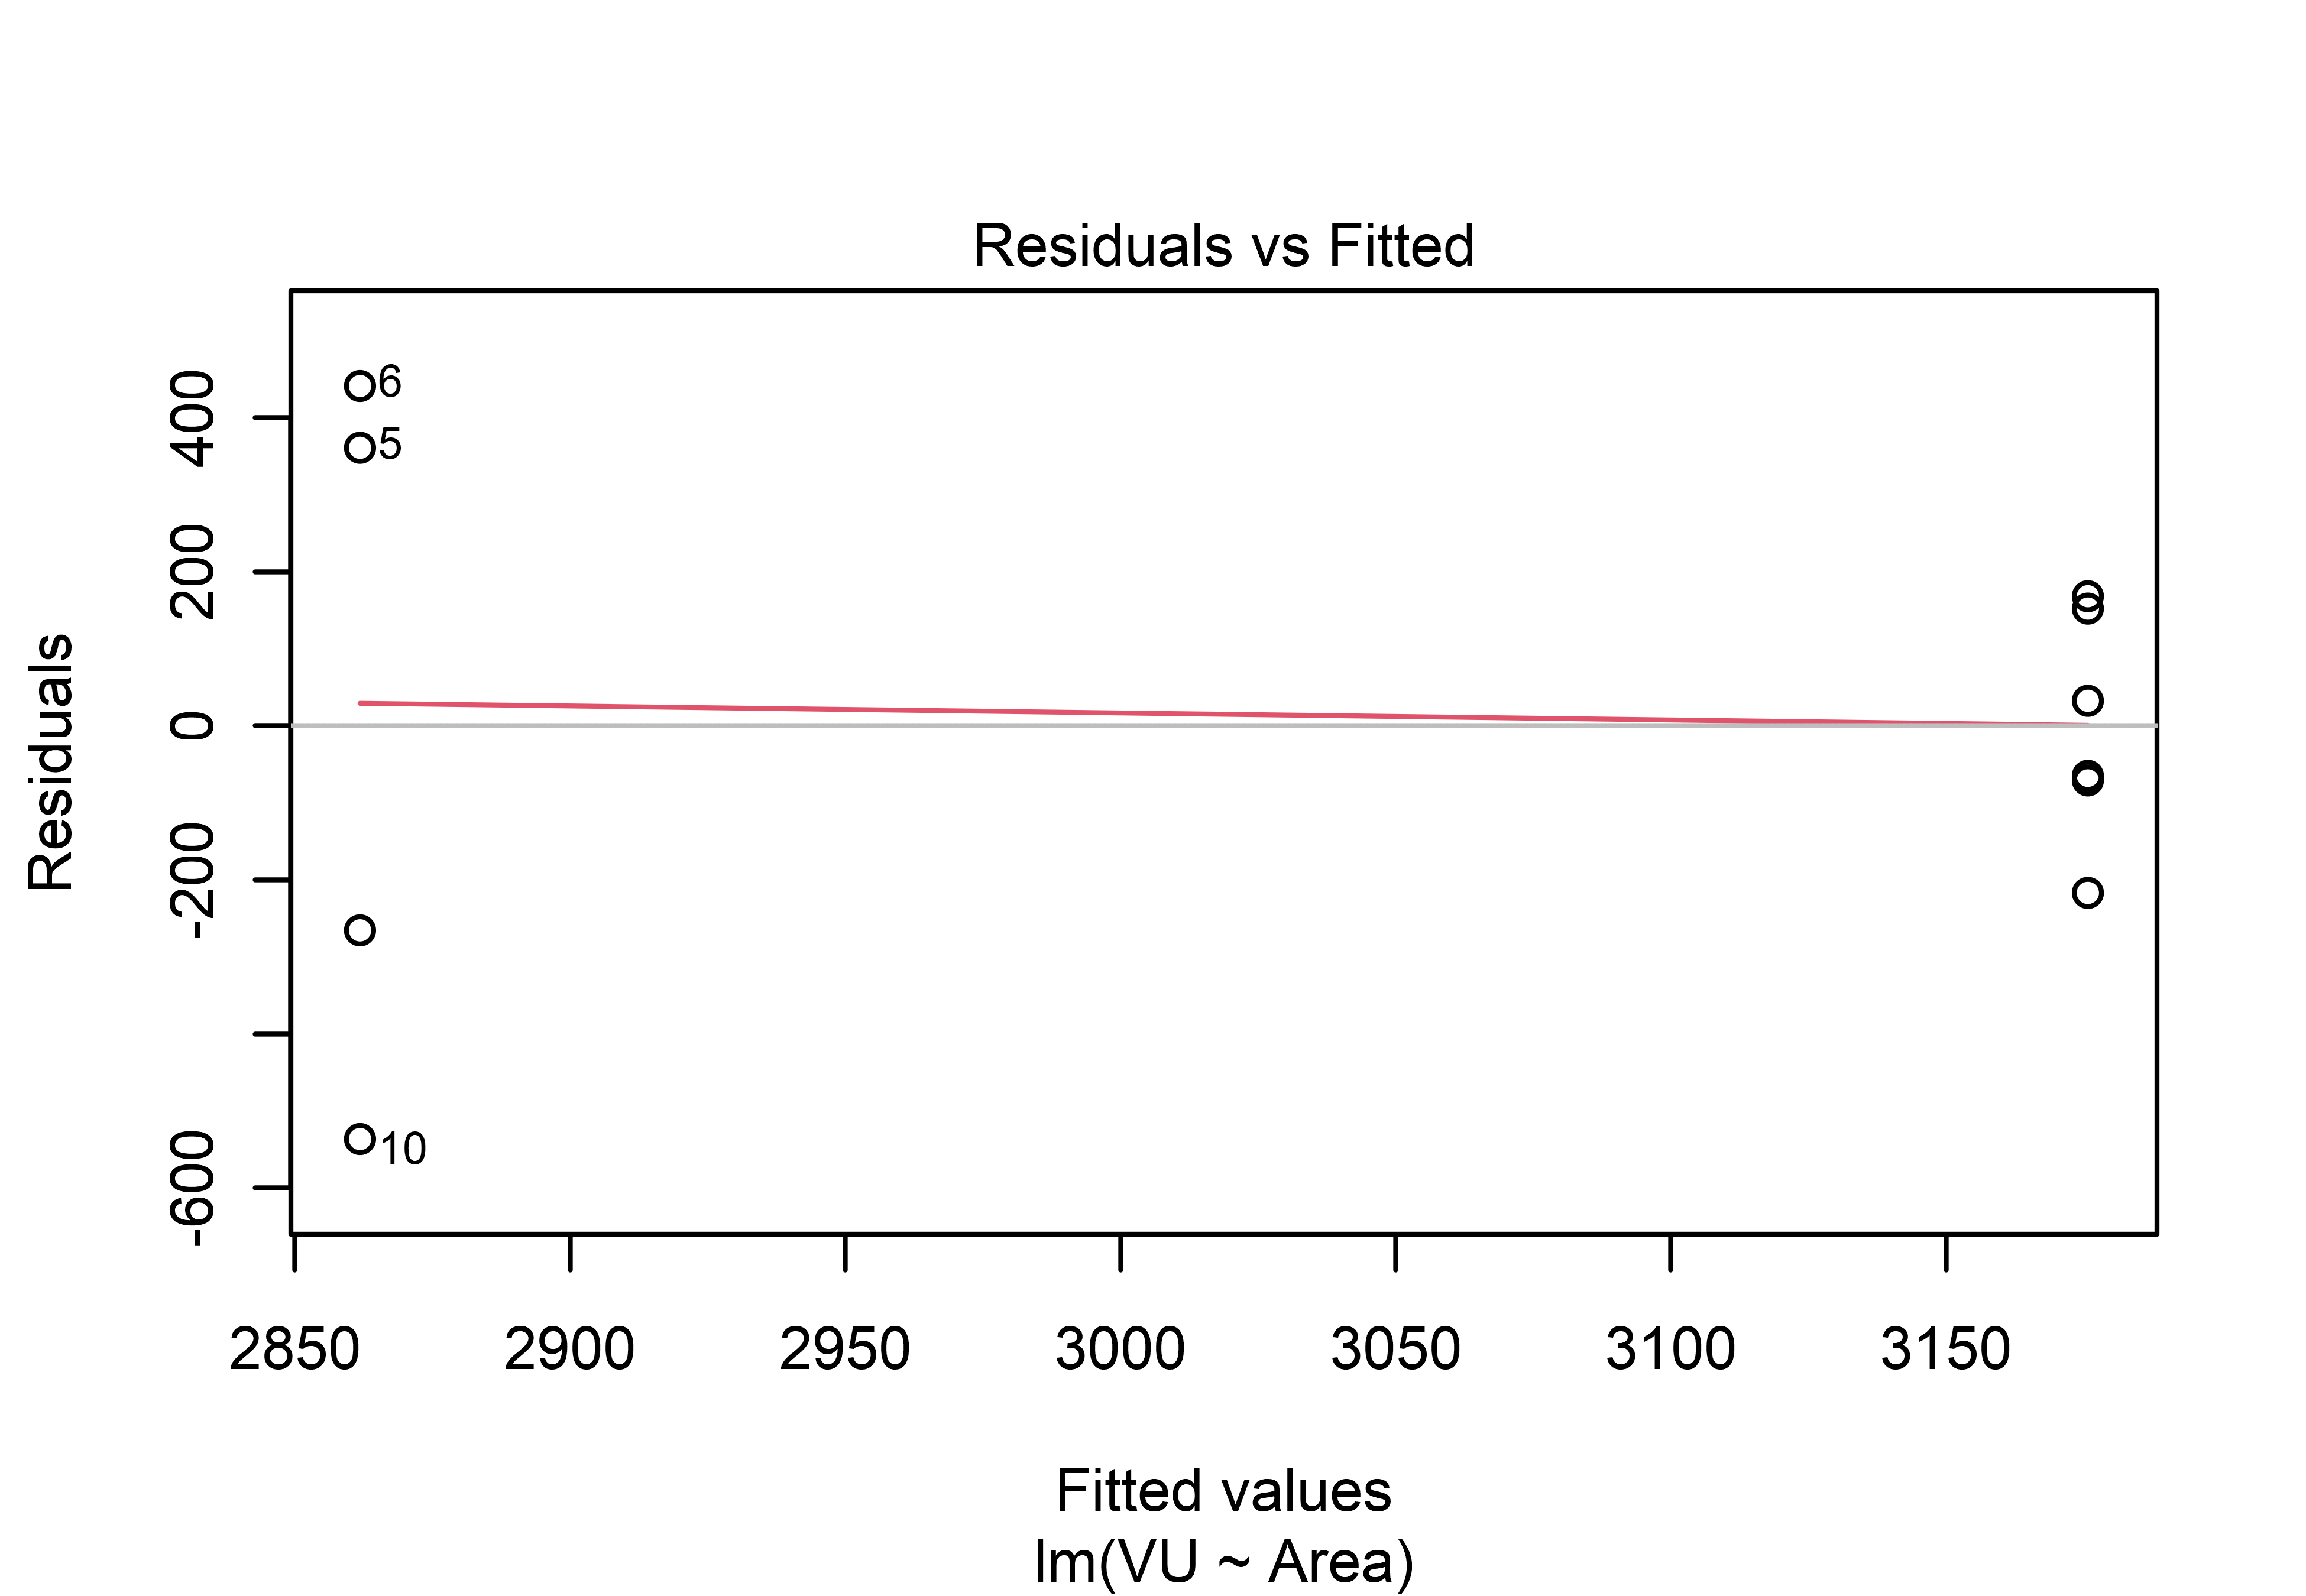
\includegraphics[width=0.65\linewidth]{images/hetero-1} 

}

\caption{Gráfico de resíduos vs. valores ajustados.}\label{fig:hetero}
\end{figure}

Ou seja, a análise dos resíduos do modelo indica uma estrutura presente
nestes resíduos. Como se sabe, esta estrutura ali presente deve-se à
variável omitida: como o modelo foi ajustado considerando dados de
diferentes características sem uma variável que represente esta mudança
de característica, o valor do coeficiente da variável \texttt{Area}
tornou-se uma espécie de média ponderada entre a redução real do valor
unitário devido ao aumento da área (para os dados de meio de quadra) e a
redução menor dos valores unitários que ocorre nos dados em situação de
esquina. Os erros, portanto, apesar de simétricos (há exatamente 2 dados
de cada característica com 480 \(m2\)) serão maiores, em magnitude, para
os imóveis de 480 \(m^2\) do que para os imóveis de 360 \(m^2\), donde
advém a heteroscedasticidade. Na segunda abordagem, como os dados em
situação de esquina foram removidos junto com a variável, este modelo
resulta homoscedástico (não mostrado).

Os intervalos de confiança e predição @80\% para os três modelos, bem
como os limites do CA podem ser vistos na tabela 9\footnote{O intervalos
  de predição para o modelo da primeira abordagem foram calculados com a
  utilização de erros robustos.} abaixo:

\begin{longtable}[]{@{}lrrrrrr@{}}
\caption{Comparação dos limites do IP e CA para os modelos do Ex.
3.}\tabularnewline
\toprule
Modelo & Estimativa central & \(IP_{inf}\) & \(IP_{sup}\) & Amplitude IP
(\%) & \(CA_{inf}\) & \(CA_{sup}\)\tabularnewline
\midrule
\endfirsthead
\toprule
Modelo & Estimativa central & \(IP_{inf}\) & \(IP_{sup}\) & Amplitude IP
(\%) & \(CA_{inf}\) & \(CA_{sup}\)\tabularnewline
\midrule
\endhead
1 & 2.984,49 & 2.466,50 & 3.502,47 & 34,71 & 2.536,81 &
3.432,16\tabularnewline
2 & 2.613,52 & 2.461,77 & 2.765,27 & 11,61 & 2.221,49 &
3.005,55\tabularnewline
3 & 3.355,45 & 3.207,46 & 3.503,44 & 8,82 & 2.852,13 &
3.858,77\tabularnewline
\bottomrule
\end{longtable}

Deve-se notar que, com a primeira abordagem, como o modelo é viesado, o
campo de arbítrio ainda resultou suficiente para absorver os efeitos da
variável omitida, o que não acontece com a segunda abordagem. Para o
terceiro modelo, novamente, as previsões centrais são boas e o IP é
pequeno.

\newpage

\hypertarget{mercado-4}{%
\subsubsection{Mercado 4}\label{mercado-4}}

\begin{wraptable}{r}{0pt}[ht]
\centering
\begin{tabular}{ccc}
  \hline
VU & Area & Situacao \\ 
  \hline
\cellcolor{gray!6}{3137} & \cellcolor{gray!6}{360} & \cellcolor{gray!6}{Meio de Quadra }\\ 
  3218 & 360 & Meio de Quadra \\ 
\cellcolor{gray!6}{  3116} & \cellcolor{gray!6}{360} & \cellcolor{gray!6}{Meio de Quadra }\\ 
  3360 & 360 & Meio de Quadra \\ 
\cellcolor{gray!6}{  4133} & \cellcolor{gray!6}{480} & \cellcolor{gray!6}{Esquina }\\ 
  4018 & 480 & Esquina \\ 
\cellcolor{gray!6}{  3249} & \cellcolor{gray!6}{360} & \cellcolor{gray!6}{Meio de Quadra }\\ 
  3274 & 360 & Meio de Quadra \\ 
\cellcolor{gray!6}{  2658} & \cellcolor{gray!6}{480} & \cellcolor{gray!6}{Meio de Quadra }\\ 
  2569 & 480 & Meio de Quadra \\ 
   \hline
\end{tabular}
\caption{Dados para o M. 4.} 
\label{tab:ex4}
\end{wraptable}

Neste quarto caso, foram seguidos exatamente os mesmos passos dos casos
anteriores. Contudo, para a geração dos valores, foi adotada uma
majoração maior para os lotes em situação de esquina, conforme
\ref{eq:ex4}, onde \(\varepsilon \sim \mathcal{N}(0, \,100^2)\) . O que
se buscou foi uma situação em que a amplitude do IP para a primeira
abordagem extrapole a amplitude do CA.

\begin{equation} \label{eq:ex4}
VU = 5000 - 5 \cdot Area + 1500 \cdot Situacao + \varepsilon
\end{equation}

Os dados gerados encontram-se na tabela \ref{tab:ex4}. Deve-se notar que
os valores das estimativas centrais para os lotes em estudo, de 480
\(m^2\), em situação de meio de quadra ou esquina, com este modelo,
serão de\\
R\$2.600,00 e R\$4.100,00, respectivamente. O que se pretende é simular
se num mercado com uma maior variabilidade o campo de arbítrio pode ser
uma bom fator limitante. Novamente, então, foram ajustados três modelos,
como os descritos no exemplo anterior.

Na tabela \ref{tab:tab4} são mostrados os coeficientes dos três modelos
ajustados. Novamente fica claro que: no primeiro modelo (coluna 1), os
coeficientes ajustados estão viesados, no segundo e no terceiro modelos
eles estão estimados corretamente, porém o terceiro modelo é mais
preciso (menores intervalos de confiança).

Deve-se notar ainda na tabela \ref{tab:tab4} que o modelo da primeira
abordagem, visto na coluna (1), apresentou coeficiente de ajuste
baixíssimo e coeficiente de correlação ajustado negativo. É possível
mostrar que, de acordo com o teste de Breusch-Pagan, a hipótese da
homoscedasticidade não pode ser verificada. O teste de significância da
variável independente do modelo não foi significante nem para enquadrar
omodelo no grau I de fundamentação da NBR 14.653-02. Ainda assim este
modelo faz boas previsões se utilizado corretamente o IP.

Já o modelo da segunda abordagem (coluna 2) tem um coeficiente de ajuste
muito alto e o modelo tem grau III de fundamentação, segundo a NBR
14.653-02. No entanto, este modelo é totalmente inadequado para fazer
previsões fora dos dados da amostra, mesmo com a utilização do CA ou do
IP.

O intervalo de predição @80\% para os três modelos, bem como os limites
do CA podem ser vistos na tabela 11\footnote{Os intervalos de predição e
  confiança para o modelo da primeira abordagem foram calculados com a
  utilização de erros robustos.} abaixo:

\begin{longtable}[]{@{}lrrrrrr@{}}
\caption{Comparação dos limites do IP e CA para os modelos do Ex.
4.}\tabularnewline
\toprule
Modelo & Estimativa central & \(IP_{inf}\) & \(IP_{sup}\) & Amplitude IP
(\%) & \(CA_{inf}\) & \(CA_{sup}\)\tabularnewline
\midrule
\endfirsthead
\toprule
Modelo & Estimativa central & \(IP_{inf}\) & \(IP_{sup}\) & Amplitude IP
(\%) & \(CA_{inf}\) & \(CA_{sup}\)\tabularnewline
\midrule
\endhead
1 & 3.344,49 & 2.344,84 & 4.344,14 & 59,78 & 2.842,81 &
3.846,16\tabularnewline
2 & 2.613,52 & 2.461,77 & 2.765,27 & 11,61 & 2.221,49 &
3.005,55\tabularnewline
3 & 4.075,45 & 3.927,46 & 4.223,44 & 7,26 & 3.464,13 &
4.686,77\tabularnewline
\bottomrule
\end{longtable}

\begin{table}[H] \centering 
  \caption{Comparação de modelos para o Ex. 4.} 
  \label{tab:tab4} 
\footnotesize 
\begin{tabular}{@{\extracolsep{5pt}}lccc} 
\\[-1.8ex]\hline 
\hline \\[-1.8ex] 
 & \multicolumn{3}{c}{\textit{Dependent variable:}} \\ 
\cline{2-4} 
\\[-1.8ex] & \multicolumn{3}{c}{VU} \\ 
\\[-1.8ex] & (1) & (2) & (3)\\ 
\hline \\[-1.8ex] 
 Constant & 2.869,4 (979,9, 4.758,8) & 5.062,3 (4.767,0, 5.357,5) & 5.062,3 (4.769,3, 5.355,3) \\ 
  & t = 1,9$^{***}$ & t = 22,0$^{***}$ & t = 22,1$^{***}$ \\ 
  Area & 1,0 ($-$4,2, 6,2) & $-$5,1 ($-$5,9, $-$4,4) & $-$5,1 ($-$5,8, $-$4,4) \\ 
  & t = 0,2 & t = $-$8,7$^{***}$ & t = $-$8,8$^{***}$ \\ 
  SituacaoEsquina &  &  & 1.461,9 (1.352,5, 1.571,4) \\ 
  &  &  & t = 17,1$^{***}$ \\ 
 \hline \\[-1.8ex] 
Observations & 10 & 8 & 10 \\ 
R$^{2}$ & 0,02 & 0,9 & 1,0 \\ 
Adjusted R$^{2}$ & $-$0,1 & 0,9 & 1,0 \\ 
Residual Std. Error & 523,0 (df = 8) & 86,1 (df = 6) & 85,4 (df = 7) \\ 
F Statistic & 0,1 (df = 1; 8) & 75,9$^{***}$ (df = 1; 6) & 148,9$^{***}$ (df = 2; 7) \\ 
\hline 
\hline \\[-1.8ex] 
Notas: & \multicolumn{3}{r}{$^{*}$p$<$0,3; $^{**}$p$<$0,2; $^{***}$p$<$0,1} \\ 
 & \multicolumn{3}{r}{Reportados erros robustos para modelo da coluna 1.} \\ 
\end{tabular} 
\end{table}

Deve-se notar que, neste mercado, como a majoração do valor unitário de
um lote devido a situação esquina é grande, com a primeira abordagem o
CA resultou insuficiente para absorver os efeitos da variável omitida. A
segunda abordagem segue com o mesmo modelo. Já com o terceiro modelo,
novamente, as previsões centrais são muito boas e o IP é pequeno.

Na primeira abordagem, deve-se notar que o IP do modelo contém o valor
`real' do lote, enquanto que o intervalo de valores dentro das
semi-amplitudes de \(\pm\) 15\% do CA não contém o valor `real' do lote,
já que o valor real do lote é \(\approx\) 29,89\% superior à estimativa
do valor central obtida com este modelo (3.344,49).

\hypertarget{suxedntese}{%
\subsubsection{Síntese}\label{suxedntese}}

Em suma, para quatro mercados diferentes (4 bairros diferentes,
digamos), foram testados três tipos de abordagens diferentes:

\begin{enumerate}
\def\labelenumi{\arabic{enumi}.}
\item
  A abordagem de se considerar todos os dados, porém excluindo a
  variável \texttt{situacao}, por conta da micronumerosidade;
\item
  A abordagem de se desconsiderar, além das variáveis, também os dados
  em situação de esquina, chegando-se assim a um modelo apenas para os
  lotes em situação de meio de quadra;
\item
  A abordagem de utilizar-se todos os dados e todas as variáveis, apesar
  disso não ir ao encontro com o estabelecido pela norma vigente, por
  conta da micronumerosidade.
\end{enumerate}

Os gráficos dos modelos para os quatro mercados podem ser vistos na
Figura \ref{fig:modelos}. Nela podem-se ver os dados do modelo
acompanhados das retas de regressão para a primeira abordagem (linha
cheia, em laranja) e para as segunda abordagem (em azul). Em cinza
pode-se ver as bandas do IP para o modelo da primeira abordagem. As
linhas laranjas tracejadas representam os limites do CA para a primeira
abordagem. Deve-se notar que, como da própria definição de IP, este
possui a propriedade de conter 80\% dos dados previstos para o mercado,
de maneira que, se a variável \texttt{Situacao} não está presente no
modelo, o IP deverá se alargar de maneira a conter 80\% dos dados. Já
num modelo ajustado com todas as variáveis relevantes, esse intervalo é
menor, já que a diferença de valores entre dados em situação de esquina
e meio de quadra seria explicada pelo efeito da variável adicional e não
seria absorvido pelos erros do modelo, como na primeira abordagem.

\begin{figure}[H]

{\centering 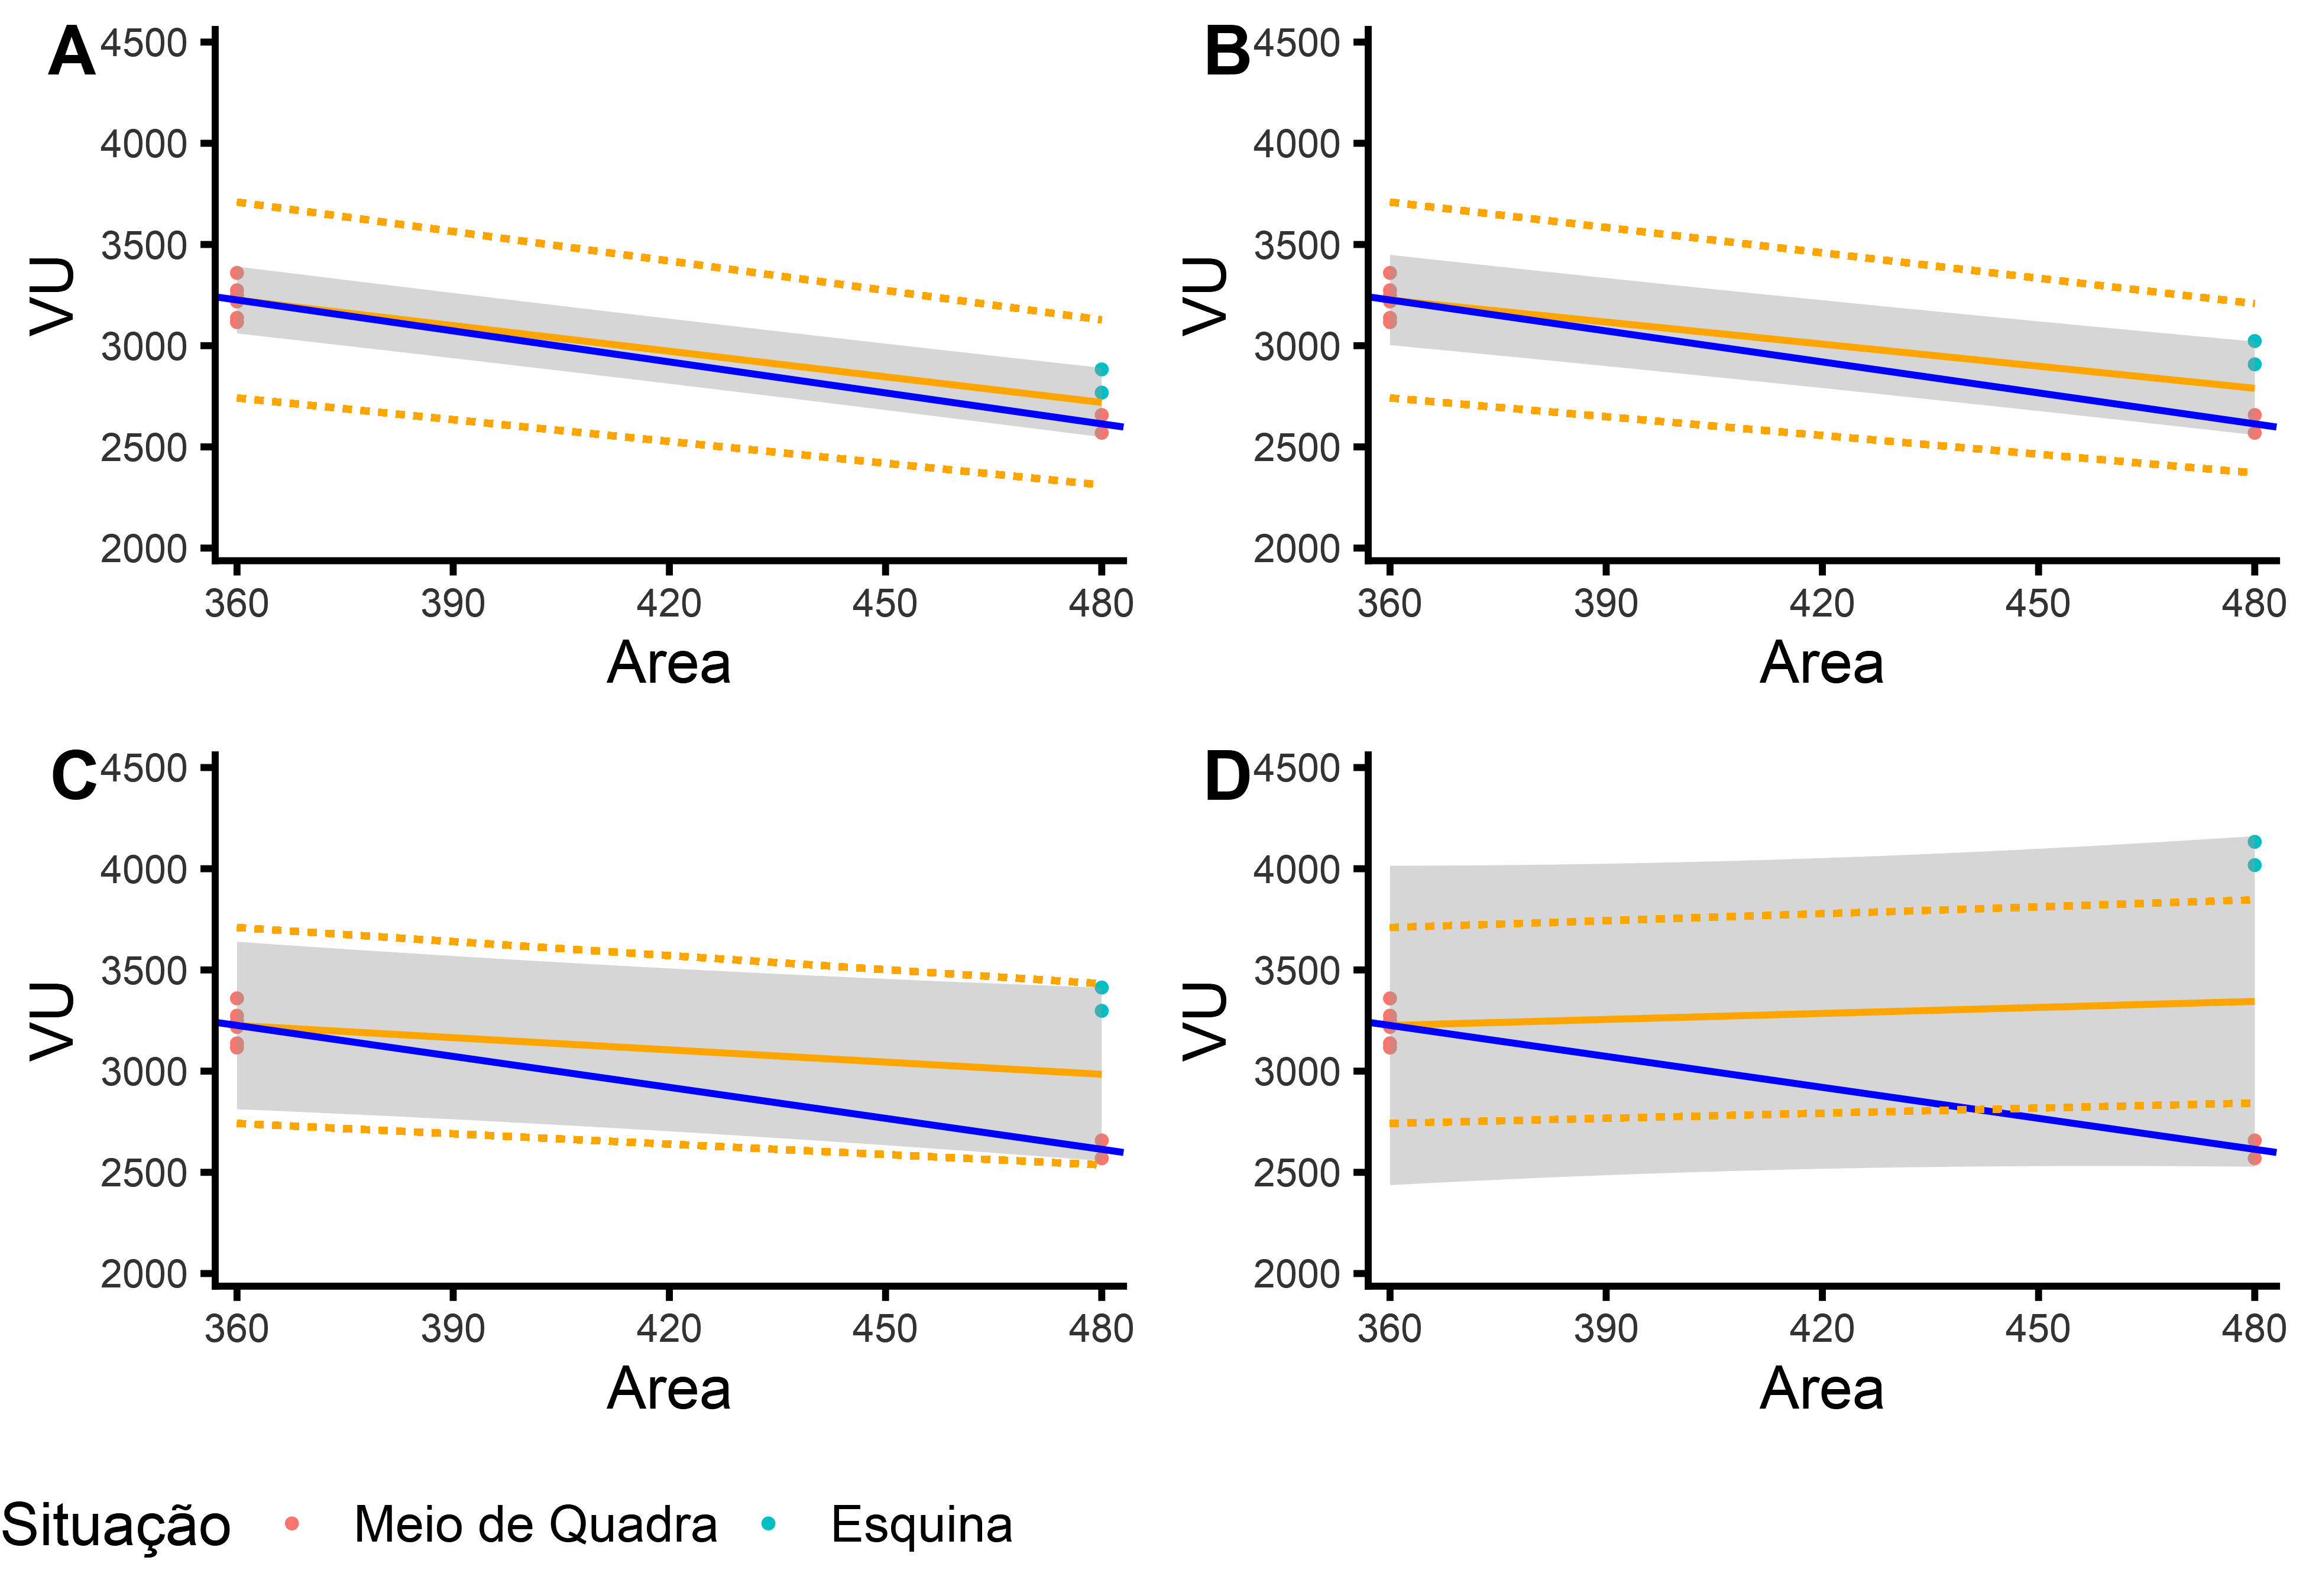
\includegraphics[width=1\linewidth]{images/modelos-1} 

}

\caption{Gráficos dos modelos para os quatro mercados.}\label{fig:modelos}
\end{figure}

Em todos os mercados (bairros) \textbf{a terceira abordagem mostrou-se
superior}, obtendo-se um valor de estimativa central mais próxima do
valor ``real'', e um IP mais estreito, além de um modelo com estimação
adequada para os coeficientes.

\begin{table}

\caption{\label{tab:comparacao}IP vs. CA em vários mercados, com diferentes abordagens.}
\centering
\begin{tabular}[t]{>{}lrrrrr}
\toprule
\multicolumn{1}{c}{\textbf{ }} & \multicolumn{1}{c}{\textbf{ }} & \multicolumn{3}{c}{\textbf{Estimativa}} & \multicolumn{1}{c}{\textbf{ }} \\
\cmidrule(l{3pt}r{3pt}){3-5}
\textbf{Mercado} & \textbf{Abordagem} & \textbf{Central} & \textbf{IP superior} & \textbf{CA superior} & \textbf{Valor 'real'}\\
\rowcolor{gray!6}
\midrule
 & 1 & 2.719,5 & 2.890,5 & 3.127,4 & \\
\cmidrule{2-5}
\rowcolor{gray!6}
 & 2 & 2.613,5 & 2.765,3 & 3.005,5 & \\
\cmidrule{2-5}
\rowcolor{gray!6}
\multirow{-3}{*}{\raggedright\arraybackslash \textbf{A}} & 3 & 2.825,5 & 2.973,4 & 3.249,3 & \multirow{-3}{*}{\raggedleft\arraybackslash 2.850}\\
\cmidrule{1-6}
 & 1 & 2.789,5 & 3.057,4 & 3.207,9 & \\
\cmidrule{2-5}
 & 2 & 2.613,5 & 2.765,3 & 3.005,5 & \\
\cmidrule{2-5}
\multirow{-3}{*}{\raggedright\arraybackslash \textbf{B}} & 3 & 2.965,5 & 3.113,4 & 3.410,3 & \multirow{-3}{*}{\raggedleft\arraybackslash 2.990}\\
\cmidrule{1-6}
\rowcolor{gray!6}
 & 1 & 2.984,5 & 3.502,5 & 3.432,2 & \\
\cmidrule{2-5}
\rowcolor{gray!6}
 & 2 & 2.613,5 & 2.765,3 & 3.005,5 & \\
\cmidrule{2-5}
\rowcolor{gray!6}
\multirow{-3}{*}{\raggedright\arraybackslash \textbf{C}} & 3 & 3.355,5 & 3.503,4 & 3.858,8 & \multirow{-3}{*}{\raggedleft\arraybackslash 3.380}\\
\cmidrule{1-6}
 & 1 & 3.344,5 & 4.344,1 & 3.846,2 & \\
\cmidrule{2-5}
 & 2 & 2.613,5 & 2.765,3 & 3.005,5 & \\
\cmidrule{2-5}
\multirow{-3}{*}{\raggedright\arraybackslash \textbf{D}} & 3 & 4.075,5 & 4.223,4 & 4.686,8 & \multirow{-3}{*}{\raggedleft\arraybackslash 4.100}\\
\bottomrule
\end{tabular}
\end{table}

Com a \textbf{segunda abordagem}, obtem-se sempre o mesmo modelo, com
mesmos intervalos de predição e mesmos campos de arbitrio, haja vista
que o que se altera nos três mercados é apenas o efeito de majoração
devido à situação de esquina, cujos dados são excluídos nesta abordagem.
Apesar deste modelo obter coeficientes ajustados corretamente para as
demais variáveis, ele não é bom para se efetuar previsões para dados com
características diferentes dos dados efetivamente utilizados na amostra.
A adoção do CA ou do IP só pode ser feita completamente no escuro, sem
que exista nada que possa embasar a magnitude da majoração dos valores
das estimativas centrais, que são válidas apenas para os tipos de dados
permanecentes na amostra, no caso, os dados em situação de meio de
quadra.

Finalmente, com a \textbf{primeira abordagem}, apesar dos coeficientes
serem estimados de maneira muito pobre, viesados por conta do efeito da
variável relevante omitida, o modelo obtido é razoavelmente bom para
fazer previsões, desde que se faça o uso correto do intervalo de
predição. Deve-se ter em mente que o modelo não prevê como estimativa de
valor central nem o valor para o lote em situação de meio de quadra, nem
o valor do lote em situação de esquina, mas algo entre as duas
situações. Para se prever valores dos lotes de meio de quadra deve-se
minorar os valores das estimativas centrais enquanto que para os lotes
de esquina, deve-se majorá-las\footnote{Essentially, all models are
  wrong, but some are useful (BOX; DRAPER,
  \protect\hyperlink{ref-Box1986}{1986}, p. 424).}.

\begin{longtable}[]{@{}crrr@{}}
\caption{Erros (\%) obtidos com a utilização da segunda
abordagem.}\tabularnewline
\toprule
Mercado & Erro \(\hat Y\) & Erro \(\hat Y_{sup}\) & Erro
\(CA_{sup}\)\tabularnewline
\midrule
\endfirsthead
\toprule
Mercado & Erro \(\hat Y\) & Erro \(\hat Y_{sup}\) & Erro
\(CA_{sup}\)\tabularnewline
\midrule
\endhead
A & -8,30\% & -2,97\% & 5,46\%\tabularnewline
B & -12,59\% & -7,52\% & 0,52\%\tabularnewline
C & -22,68\% & -18,19\% & -11,08\%\tabularnewline
D & -36,26\% & -32,55\% & -26,69\%\tabularnewline
\bottomrule
\end{longtable}

Com a adoção do limite superior do IP, porém, o erro cometido com a
primeira abordagem é muito pequeno, independente do mercado estudado,
como ilustra a tabela abaixo. Os erros que se cometeriam ao se utilizar
o limite superior do CA, comum na prática da engenharia de avaliações, é
muito maior do que o erro cometido com a adoção do limite superior do
IP.

\begin{longtable}[]{@{}crrr@{}}
\caption{Erros (\%) obtidos com a utilização da primeira
abordagem.}\tabularnewline
\toprule
Mercado & Erro \(\hat Y\) & Erro \(\hat Y_{sup}\) & Erro
\(CA_{sup}\)\tabularnewline
\midrule
\endfirsthead
\toprule
Mercado & Erro \(\hat Y\) & Erro \(\hat Y_{sup}\) & Erro
\(CA_{sup}\)\tabularnewline
\midrule
\endhead
A & -4,58\% & 1,42\% & 9,73\%\tabularnewline
B & -6,71\% & 2,25\% & 7,29\%\tabularnewline
C & -11,70\% & 3,62\% & 1,54\%\tabularnewline
D & -18,43\% & 5,95\% & -6,19\%\tabularnewline
\bottomrule
\end{longtable}

\newpage

\hypertarget{estudo-de-caso-2-avaliauxe7uxe3o-intervalar}{%
\subsection{Estudo de Caso 2 -- Avaliação
intervalar}\label{estudo-de-caso-2-avaliauxe7uxe3o-intervalar}}

No estudo de caso anterior trabalhou-se com o problema da omissão de
variável relevanto no modelo. No presente estudo de caso será averiguada
a previsão de valores e avaliação de intervalos admissíveis, devido ao
efeito de variáveis não-relevantes, isto é, variáveis que agregariam
pouco grau de explicação ao modelo. Como foi visto na revisão
bibliográfica, não se pode acrescentar tantas variáveis quanto se deseje
a um modelo, já que isso poderia levar a um superajuste do modelo, que
seria bom para explicar a amostra de trabalho, mas não o mercado em
análise. Desta forma, os (pequenos) efeitos destas variáveis ausentes
são absorvidos pelo termo de erro, o que é desejado.

Imagine-se, então, que durante a construção de um modelo sobre uma
amostra de mercado de apartamentos em uma zona central de uma cidade
qualquer, não foram incluídas no modelo uma série de variáveis que,
apesar dos seus pequenos efeitos, acabam por impactar de alguma forma na
formação de preço dos apartamentos (melhor posição solar, melhor
ventilação, melhor vista), já que o número de dados da amostra é
limitado.

Porém, um avaliador experiente, ciente das limitações do seu modelo,
durante a avaliação de um apartamento nesta zona central, se deparou com
o seguinte problema: o imóvel avaliando possuía, para todas as
características não contempladas no modelo, valores acima da média. Por
exemplo, imagine-se que o imóvel avaliando possuía uma vista
privilegiada, uma melhor posição solar e ainda melhor posição em relação
aos ventos, de tal maneira que, ao se avaliar tal imóvel pelo valor
médio calculado pelo modelo estaria-se notoriamente sub-avaliando o
mesmo. No estudo de caso anterior, a utilização do Campo de Arbítrio do
Avaliador era possível, já que \emph{variáveis relevantes} não foram
\emph{contempladas no modelo }. Neste caso, porém, o problema é diverso:
o imóvel avaliando não vale mais porque houve a omissão de uma variável
relevante, mas sim por uma soma de pequenos efeitos que, somados,
tornaram-se relevantes.

Para melhor ilustrar foram simulados dados conforme a equação
\ref{eq:ex5}, onde \(Padrao_j\) é uma variável qualitativa (dicotômica
em grupo) com níveis \(j\) variando de 1 a 5 (muito baixo, baixo, médio,
alto e muito alto) e \(\varepsilon \sim \mathcal{N}(0, \,100^2)\) . Os
gráficos do modelo ajustado com os dados simulados podem ser vistos na
Figura \ref{fig:modelo}.

\begin{equation} \label{eq:ex5}
VU = 5000 - 5 \cdot Area + 250 \cdot Padrao_j + \varepsilon
\end{equation}

\begin{figure}[H]

{\centering 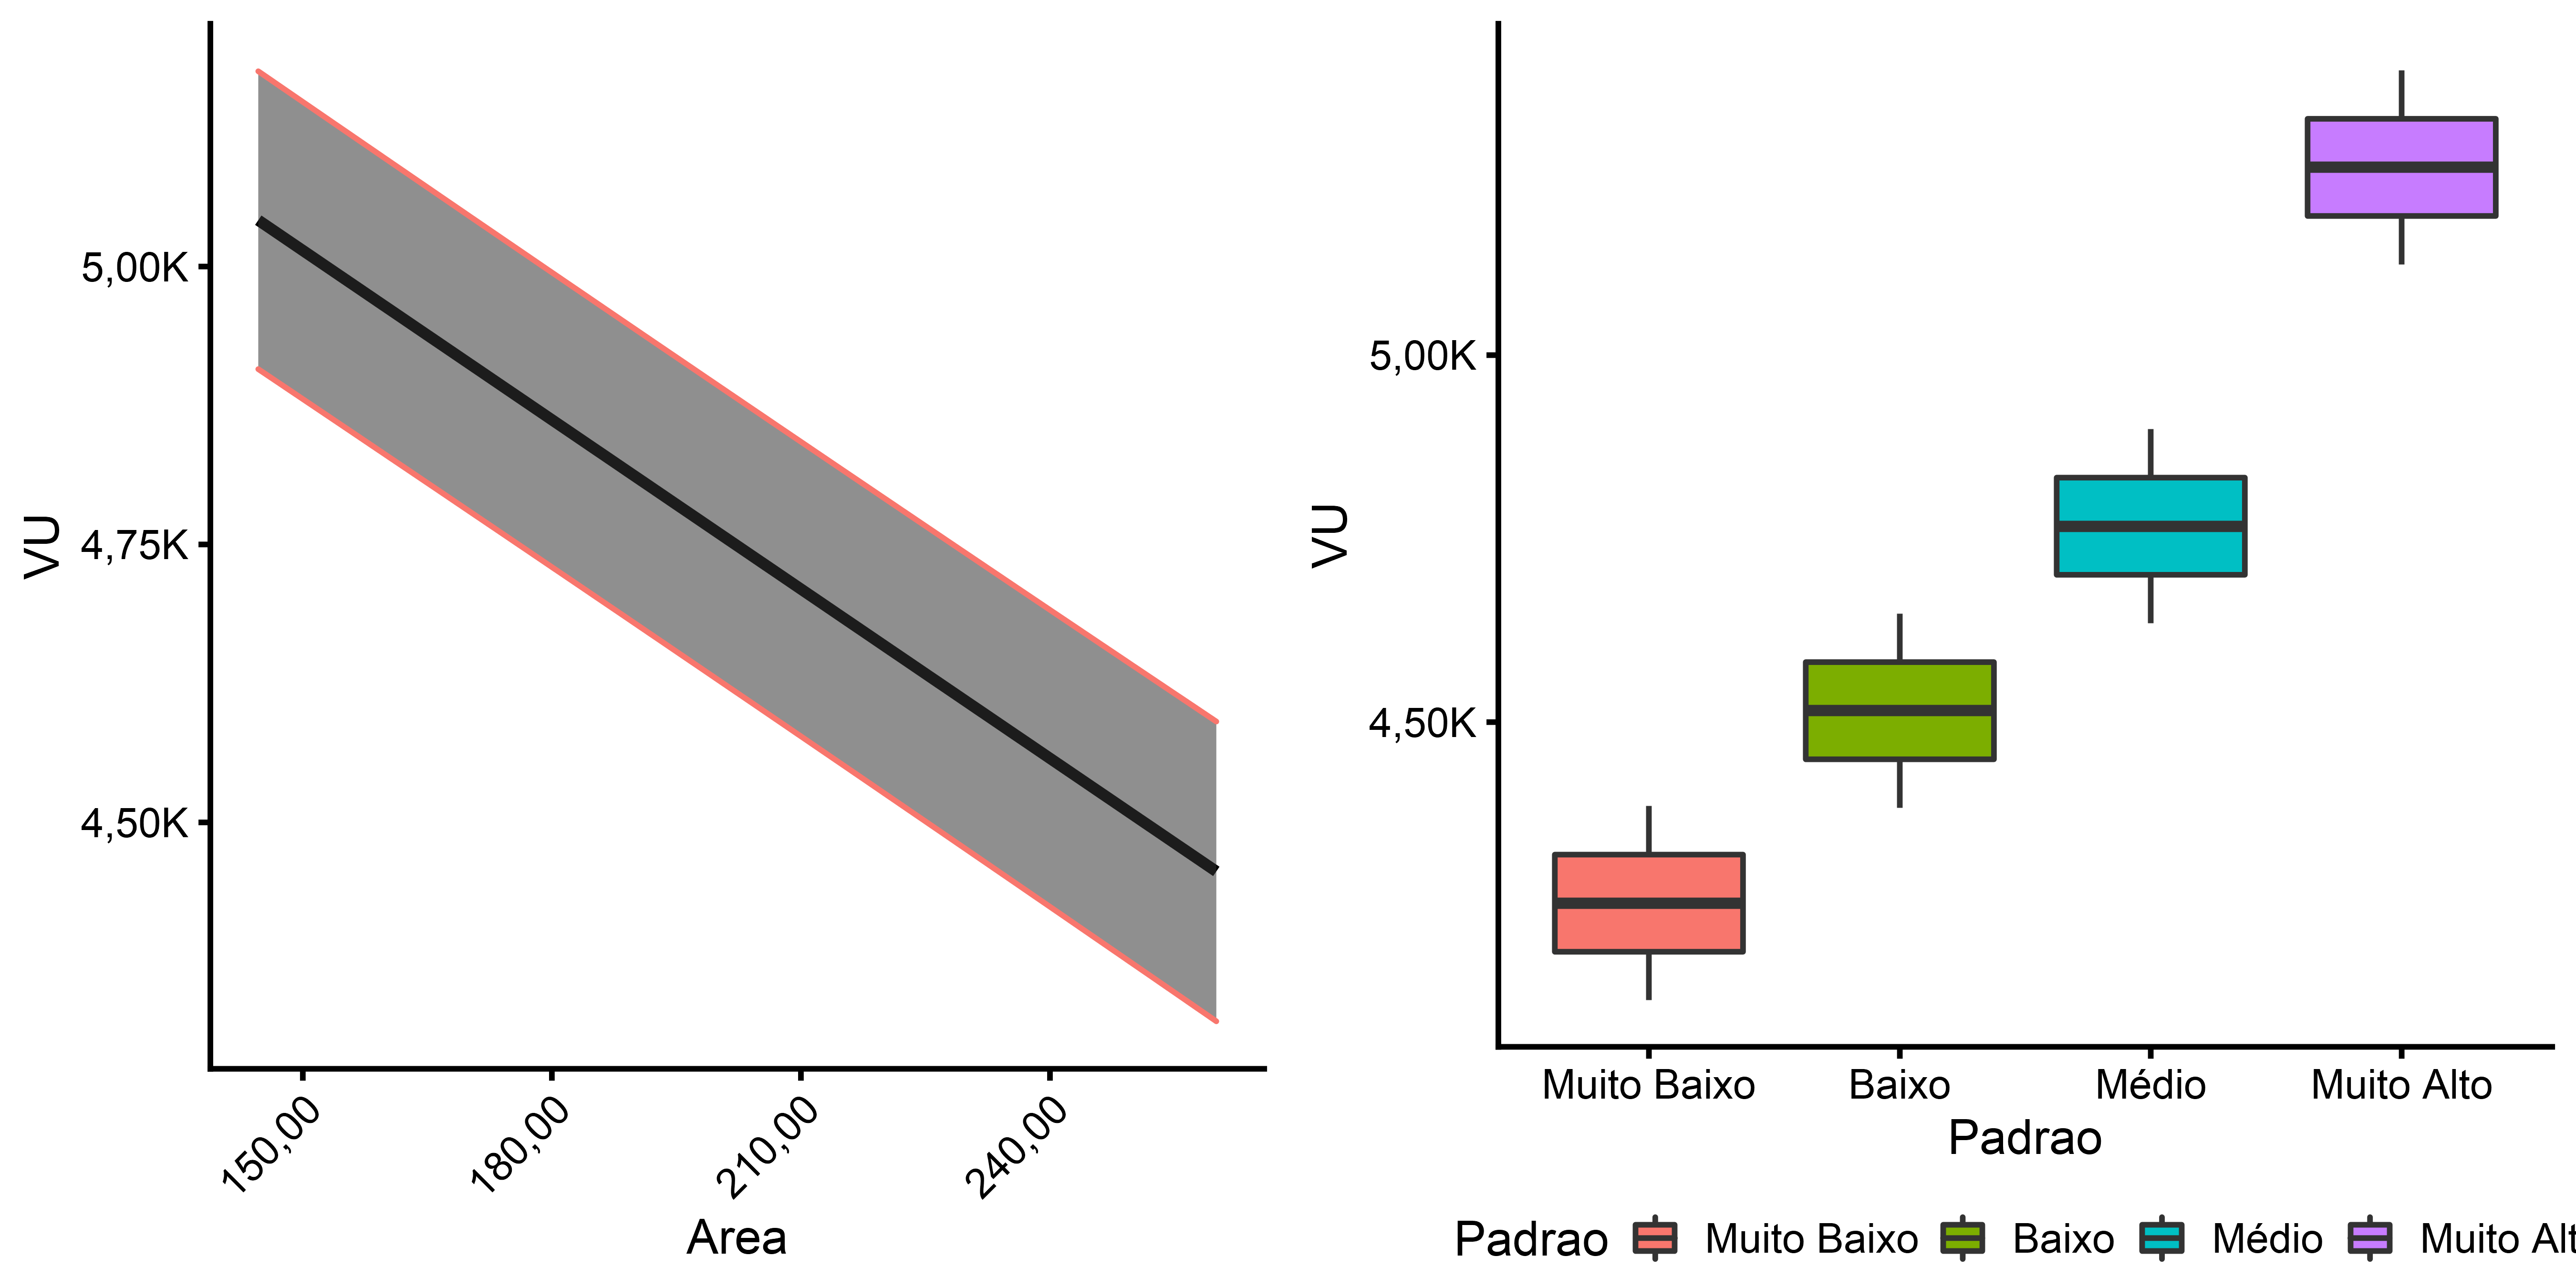
\includegraphics[width=0.7\linewidth]{images/modelo-1} 

}

\caption{Modelo ajustado para apartamentos.}\label{fig:modelo}
\end{figure}

Imagine-se agora que o imóvel avaliando conta com área de 200 \(m^2\) e
padrão médio (3). O valor da estimativa central para este imóvel, com
este modelo, seria de R\$ 5.014,43.\footnote{Intervalo de confiança:
  {[}4.988,17, 5.040,68{]}}Imagine-se agora que o avaliador, convicto
que o valor do imóvel encontra-se acima do valor médio previsto para o
modelo para um imóvel com aquelas características, resolveu adotar, para
o imóvel-avaliando o valor do limite superior do intervalo de predição.
Para os dados simulados, este valor seria igual a 5.148,07. Qual seria,
então, um intervalo razoável de valores admissíveis?

Como limite inferior, pode-se dizer que, muito provavelmente, o imóvel
não está abaixo da média para aquele padrão.\footnote{Não faz qualquer
  sentido, se o avaliador arbitra um valor acima da média para o
  bem-avaliando, depois reportar como admissível um valor abaixo da
  média! Atualmente, isto é possível, conforme Figura A.2 da NBR
  14.653-02 (\protect\hyperlink{ref-NBR1465302}{2011}).} Logo, o limite
inferior do IC para a estimativa de valor central seria um bom indicador
de um limite inferior para os valores admissíveis. E quanto ao limite
superior admissível? Neste caso, seria razoável adotar o limite superior
do CA. Já que a NBR não permite que se extrapole os 15\% do CA, este é o
limite superior do intervalo. Caso o limite superior do IP ultrapasse os
15\%, esta arbitragem não seria aceita, mas caso o limite superior do IP
esteja dentro do CA, é razoável que o intervalo de valores admissíveis
esteja entre o valor central e o limite superior do CA. Em suma,
adotando-se estes critérios, o intervalor de valores admissíveis seria
coerente, apesar de altamente assimétrico : 4.988,17 \(\leq\) 5.148,07
\(\leq\) 5.766,59

Outra opção seria adotar um intervalo admissível sempre simétrico, com
semi-amplitude igual à menor distância entre: a) o valor adotado e o
valor central, ou; b) o valor adotado e o limite superior/inferior do
CA. Parte-se do pressuposto que o valor arbitrado é considerado o mais
provável pelo avaliador, sendo que, em direção aos dois extremos, a
probabilidade de ocorrência de valor diminui simetricamente.Neste caso,
o avaliador obteria, com este modelo, o seguinte intervalo de valores
admissíveis: 4.988,17 \(\leq\) 5.148,07 \(\leq\) 5.307,97

Os dois intervalos podem ser visualizados nas áreas em azul claro na
Figura \ref{fig:dists} A (assimétrico) e B (simétrico):

\begin{figure}[H]

{\centering 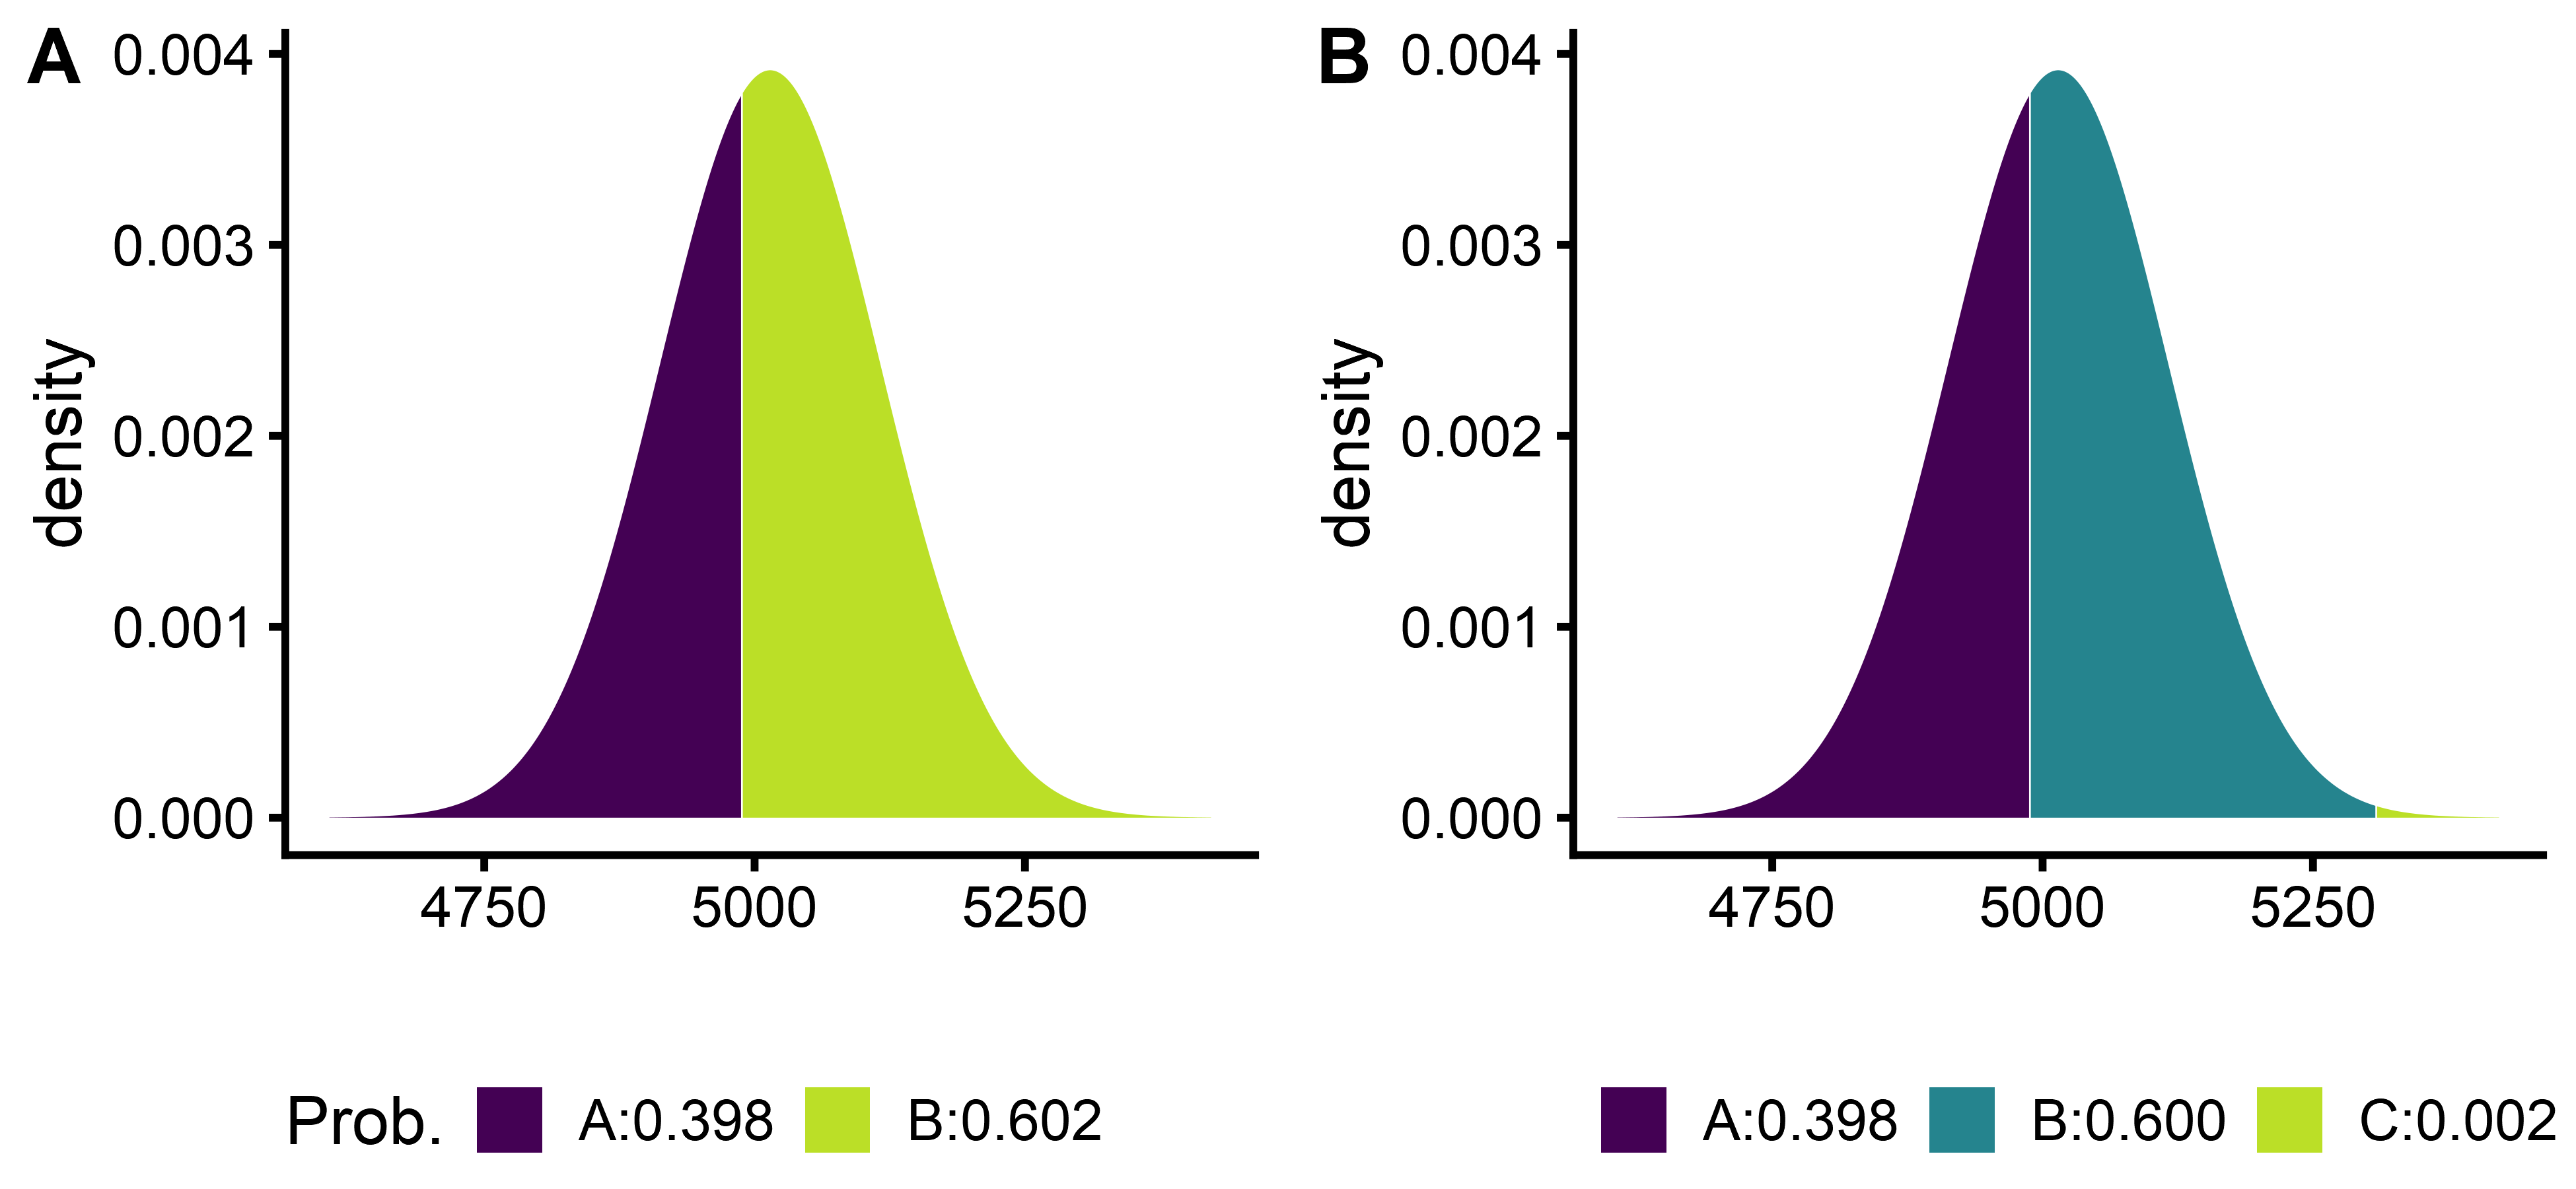
\includegraphics[width=1\linewidth]{images/dists-1} 

}

\caption{Distribuição de probabilidades dos intervalos sugeridos.}\label{fig:dists}
\end{figure}

Em suma, acredita-se que uma boa melhoria em termos de normatização
seria obtida se a NBR 14.653 estabelecesse que, para o caso da
arbitragem de valores (fora da estimativa central) esta seja feita
dentro do IP e do CA, simultaneamente. Além disto, que seja reportado um
intervalo de valores admissíveis coerente, conforme proposto acima.

Resta, porém, a solução de um outro problema: como foi visto na Figura
\ref{fig:modelo}, os dados para este exemplo ainda foram modelados com
uma dificuldade adicional, pois não foram inclusos, propositalmente,
dados de um padrão em especial, a saber, dados de imóveis de padrão alto
(foram excluídos os dados simulados com esta característica na confecção
do modelo, visando simular que os dados com esta características
apresentavam micronumerosidade).

A supressão destes dados ao modelo deixa o avaliador sem condições de
utilizá-lo para fins de avaliação de imóveis com estas
características.\footnote{Seria possível modelar a variável com um
  código alocado e interpolar, mas não é possível fazer isto para
  variáveis dicotômicas em grupo.} Se o avaliador inclui os dados com
aquelas características, ainda que em situação de micronumerosidade, ele
poderá fazer previsões para os imóveis com aquela característica, ainda
que menos precisas que as previsões feitas para as demais
características, com número maior de dados. É o que se nota na Figura
\ref{fig:modelo1}: para a característica 4 (padrão alto), o IP é maior
do que para as outras características, ou seja, as previsões obtidas com
este modelo para imóveis com estas características serão menos
confiáveis, mas ainda assim é melhor do que não poder obter previsão
alguma. Pode ser, ainda, que as previsões assim obtidas sejam melhores
do que as que se obteriam com a interpolação numa variável de código
alocado. Mais uma vez, entende-se que seria melhor deixar o modelo
falar: se o intervalo de predição encontrado for muito grande, maior do
que o CA, descarta-se a utilização do modelo. Se for menor do que o CA,
por que não utilizá-lo?

\begin{figure}[H]

{\centering 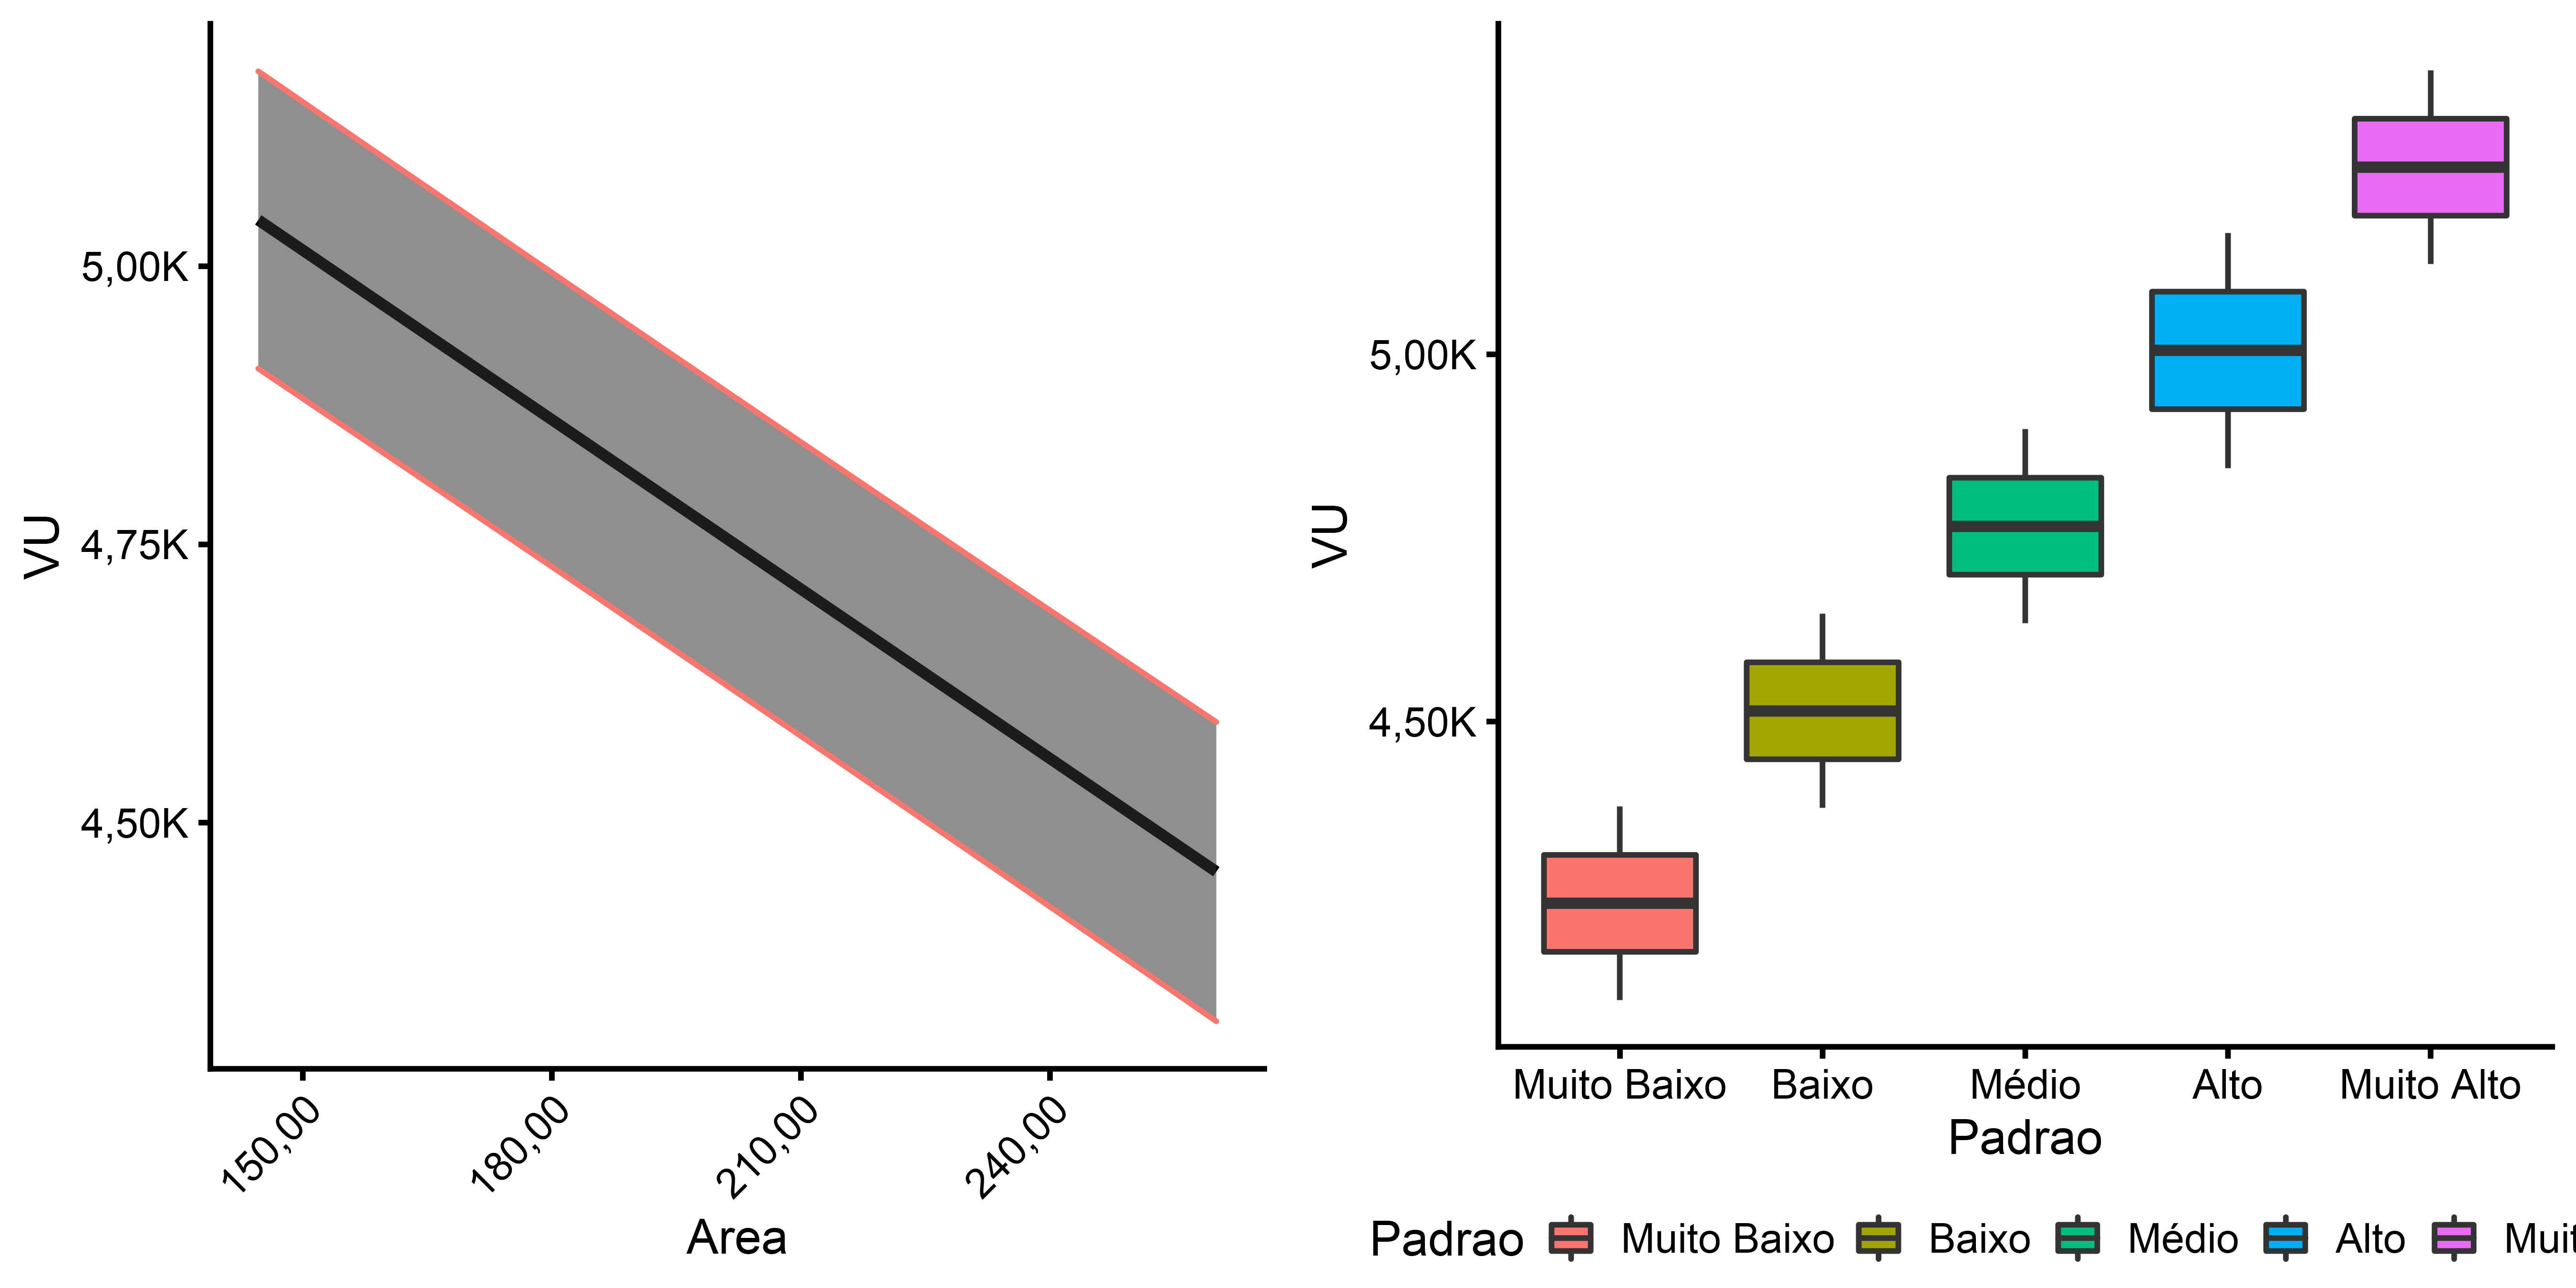
\includegraphics[width=0.7\linewidth]{images/modelo1-1} 

}

\caption{Modelo com dados em micronumerosidade.}\label{fig:modelo1}
\end{figure}

\hypertarget{conclusuxe3o-e-recomendauxe7uxf5es}{%
\section{Conclusão e
Recomendações}\label{conclusuxe3o-e-recomendauxe7uxf5es}}

Primeiramente, deve-se concluir que a micronumerosidade é um critério
que deveria ser menos rigoroso na normatização. A presença de poucos
dados pode fazer com que a estimação não seja tão boa, porém a retirada
de dados ou omissão de variáveis relevantes pode ser ainda pior. A
princípio, a norma deveria deixar o modelo dizer se a quantidade de
dados é suficiente ou não: no caso da variável apresentar significância
estatística, por que removê-la? Além do mais, dados preciosos podem
estar sendo jogados fora (no exemplo, 20\% deles), o que faz com que a
estimação dos outros coeficientes do modelo piorar.

A opção de apenas remover a variável, mantendo-se os dados, pode ser
feita, mas com o devido cuidado: o(s) valor(es) do(s) coeficiente(s)
estimados para a(s) variável(eis) efetivamente utilizada(s) deve(m) ser
visto(s) com ressalvas, pois nele(s) estão embutidos os efeitos da
variável omitida. Além do mais, para que isto seja possível, é
necessário rever outros itens da NBR 14.653-02, relacionados aos desvios
em relação às hipóteses da inferência clássica: com a omissão de
variável relevante, conforme demonstrado, o esperado é que algumas
hipóteses sejam violadas, mas isto não é impeditivo da utilização do
modelo: a utilização de erros robustos (Eicker-White) para estimar os
intervalos de confiança e predição podem solucionar o problema a
contento (ver ZONATO et al., \protect\hyperlink{ref-zonato2018}{2018}).
É necessário, contudo, normatizar este procedimento.

Com relação ao Campo de Arbítrio do Avaliador, a princípio entende-se
que este deva ser mantido na NBR 14.653-02, até por compatilidade com as
outras partes da NBR 14.653, mas também por compatibilidade com os
outros métodos, como os métodos de avaliação por fatores. A sua
aplicação, contudo, deveria ser revista: primeiramente, entende-se que é
um erro a livre utilização de todo o intervalo do CA sem um critério que
possa dar embasamento a esta utilização. A amplitude máxima do CA
deveria ser mantida, porém como limitante superior/inferior para os
intervalos de valores admissíveis, não como uma opção de livre escolha
para o avaliador arbitrar qualquer valor dentro deste intervalo, como
ocorre na atual normatização. Entende-se que seria boa regra permitir ao
avaliador que arbire valores limitados simultaneamente pelo CA e pelo
IP, utilizando os limites destes intervalos como limites do intervalo de
valores admissíveis, deixando claro que a probabilidade de ocorrência
diminui (simetricamente) à medida que se afasta do valor arbitrado.

\hypertarget{referuxeancias}{%
\section*{Referências}\label{referuxeancias}}
\addcontentsline{toc}{section}{Referências}

\hypertarget{refs}{}
\leavevmode\hypertarget{ref-NBR1465302}{}%
ABNT. \textbf{NBR 14653-2: Avaliação de bens -- parte 2: Imóveis
urbanos}. Rio de Janeiro: Associação Brasileira de Normas Técnicas,
2011.

\leavevmode\hypertarget{ref-Box1986}{}%
BOX, G. E. P.; DRAPER, N. R. \textbf{Empirical model-building and
response surface}. New York, NY, USA: John Wiley \& Sons, Inc., 1986.

\leavevmode\hypertarget{ref-droubi2019}{}%
DROUBI, L. F. P.; ZILLI, C. A.; ZONATO, W.; HOCHHEIM, N. Crítica à
avaliação intervalar na NBR 14.653-02. In: XX Congresso Brasileiro de
Avaliações e Perícias. \textbf{Anais\ldots{}}, 2019. Florianópolis:
COBREAP.

\leavevmode\hypertarget{ref-horowitz}{}%
HOROWITZ, J. L. The role of the list price in housing markets: Theory
and an econometric model. \textbf{Journal of Applied Econometrics}, v.
7, n. 2, p. 115--129, 1992. Disponível em:
\textless{}\url{https://onlinelibrary.wiley.com/doi/abs/10.1002/jae.3950070202}\textgreater..

\leavevmode\hypertarget{ref-matloff2017}{}%
MATLOFF, N. \textbf{Statistical regression and classification: From
linear models to machine learning}. Boca Raton, Florida: Chapman \&
Hall, 2017.

\leavevmode\hypertarget{ref-ASA}{}%
WASSERSTEIN, R. L.; LAZAR, N. A. The ASA's statement on p-values:
Context, process, and purpose. \textbf{The American Statistician}, v.
70, n. 2, p. 129--133, 2016. Taylor \& Francis. Disponível em:
\textless{}\url{https://doi.org/10.1080/00031305.2016.1154108}\textgreater..

\leavevmode\hypertarget{ref-zonato2018}{}%
ZONATO, W.; DROUBI, L. F. P.; HOCHHEIM, N. Pressupostos clássicos dos
modelos de regressão linear e suas implica ções sobre as avaliações em
massa. In: 13º Congresso Brasileiro de Cadastro Técnico Multifinalitário
e Gestão Territorial. \textbf{Anais\ldots{}}, 2018. Florianópolis:
COBRAC.

\end{document}
